\documentclass[preprint,review,fleqn,sort&compress,3p]{elsarticle}
\usepackage{mathrsfs}
\usepackage{adjustbox}
\usepackage{amsfonts}
\usepackage{color}
\usepackage{graphicx}
\usepackage{epstopdf}
\usepackage{amssymb}
\usepackage{amsthm}
\usepackage{amsmath}
\usepackage{bbm}
\usepackage{booktabs}
\usepackage{makecell}
\usepackage{float}
\usepackage{multirow}
\usepackage{pifont}
\usepackage{tabularx}
\usepackage{subfigure}
\usepackage{stfloats}
\usepackage{ragged2e} 
\usepackage{comment}

\theoremstyle{definition} % 这会让环境内容为正体
\newtheorem*{definition}{Definition}

\usepackage[
pdfauthor={Xiaoqing Li, Haoxiang Zhao, Liang Han, Jun Cheng, Kaibo Shi},
pdftitle={Adaptive Event-Triggered H-infinity Control for Interval Type-2 Fuzzy Cyber-Physical Systems Under Deception Attacks and Actuator Failures},
pdfstartview=XYZ,
bookmarks=true,
colorlinks=true,
linkcolor=blue,
urlcolor=blue,
citecolor=blue,
pdftex,
linktocpage=true,   % makes the page number as hyperlink in table of content
hyperindex=true
]{hyperref}
\newcommand\crefrangeconjunction{--}
\usepackage{array, threeparttable}
\usepackage[font=small,labelfont=bf,labelsep=none]{caption}
\captionsetup[table]{
	labelfont = bf,    % "Table X" 加粗
	%textfont = it,     % 标题文本斜体（根据期刊要求调整）
	%labelsep=newline,%换行
	justification = centering,
	singlelinecheck = false, % 允许换行
	labelsep = period,  % 编号和标题间空格sapce,period加点,不加space、period这两个就是冒号
	skip = 6pt         % 标题与表格间距
}
\usepackage{accents}
\newcommand{\ubar}[1]{\underaccent{\bar}{#1}}

\theoremstyle{definition}%直立体
\newtheorem{thm}{Theorem}[section]
\newtheorem{pro}{proposition}[section]
\newtheorem{cor}{Corollary}[section]
\newtheorem{Lem}{Lemma}[section]
\newtheorem{Def}{Definition}[section]
\newtheorem{rem}{Remark}[section]
\newtheorem{asptn}{Assumption}[section]
\newtheorem{example}{Example}

\journal{Neural Networks}
\geometry{reset,a4paper,left=1cm,right=1cm,top=1.2cm,bottom=2cm}
\renewcommand\baselinestretch{1.0}
\linespread{1.15}

\begin{document}
	\captionsetup[figure]{labelfont={bf},labelformat={default},labelsep=period,name={Fig.}}
	\begin{frontmatter}
		
		\title{{Adaptive Event-Triggered Control for 
				Interval Type-2 Fuzzy Cyber-Physical Systems Under Deception Attacks 
				and Actuator Failures: A Membership-Function-Derivative-Dependent 
				Switching Perspective
		}}
		
		\author[a]{Xiaoqing Li\corref{cor1}}
		\author[a]{Haoxiang Zhao}
		\author[a]{Liang Han}
		\author[b]{Jun Cheng}
		\author[c]{Kaibo Shi}
		
		\address[a]{School of Electrical Engineering and Automation, Hefei University of Technology, Hefei 230009, China}
		\address[b]{College of Mathematics and Statistics, Guangxi Normal University, Guilin 541006, China}
		\address[c]{School of Electronic Information and Electrical Engineering, Chengdu University, Chengdu 610106, China}
		
		{\cortext[cor1]{Corresponding author. E-mail addresses: 
				lxiaoqing2016@126.com (Xiaoqing Li), 2025110394@mail.hfut.edu.cn (Haoxiang Zhao), 
				lianghan@hfut.edu.cn (Liang Han),
				jcheng6819@126.com (Jun Cheng), skb111@163.com (Kaibo Shi)}}
		
		%% Abstract
\begin{abstract}
This article addresses adaptive event-triggered control for interval type-2 (IT-2) fuzzy cyber-physical systems (CPSs) affected by stochastic deception attacks and Markov-type actuator failures. Since nonlinear CPSs face cyber-layer attacks as well as physical-layer component failures, while their communication resources are often limited, an adaptive event-triggered mechanism (AETM) is employed to reduce redundant network transmissions through dynamic adjustment of the triggering threshold based on real-time state-error information. Specifically, stochastic deception attacks are characterized by a Bernoulli process, and actuator failures are modeled by Markov switching fault matrices. Accordingly, a unified closed-loop model is established. Then, a looped functional dependent on fuzzy membership functions (FMFs) is constructed to exploit membership-function information and sampled-data dynamics. Based on this functional, stability criteria are obtained to guarantee asymptotic stability of the closed-loop system while achieving a prescribed $\mathrm{H}_\infty$ disturbance attenuation level. Moreover, joint design of the controller gains and adaptive triggering parameters is formulated through tractable linear matrix inequalities (LMIs). Validation is finally carried out with an engineering-motivated permanent magnet synchronous motor example and a numerical IT-2 fuzzy system to demonstrate the effectiveness and feasibility of the developed method.

\end{abstract}

\begin{keyword}
	Interval type-2 (IT-2) fuzzy cyber-physical systems (CPSs) \sep Adaptive 
	event-triggered mechanism (AETM) \sep Deception attacks \sep Markov-type actuator failures 
\end{keyword}
		
\end{frontmatter}
	
\section{Introduction}%\cite{huangReliableControlCyberphysical2019}
Driven by advances in communication, sensing, and computing, cyber-physical systems (CPSs) have attracted growing attention in modern control research. Applications of CPSs span intelligent transportation, smart grids, and advanced aviation
\cite{wangMixedVehicleGroup2024,liuFalseDataInjectionAttack2023,dingSurveyModelBasedDistributed2019}.
By integrating cyber and physical components, CPSs enable real-time monitoring and coordinated control. However, practical physical plants usually involve nonlinear dynamics, parameter perturbations, and external disturbances
\cite{chenRobustAdaptiveControl2024,yuanAdaptiveControlNonlinear2024}.
Therefore, developing control methods that can handle nonlinearities, uncertainties, and network-induced constraints is crucial to achieving reliable and stable operation of CPSs
\cite{biAdaptiveDecentralizedFiniteTime2023}.

To represent nonlinear dynamics in a tractable form, the Takagi--Sugeno (T--S)
fuzzy approach \cite{wangStabilityStabilizationTS2021,wangSwitchingAsynchronousControl2024}
is employed for nonlinear system analysis and control design. Through membership-function-based weighting of multiple local linear subsystems, T--S fuzzy models can effectively capture the behavior of complex nonlinear systems. Nevertheless, classical
T--S fuzzy models usually depend on precise membership grades, which may be
sensitive to parameter perturbations and measurement uncertainty. IT-2 fuzzy systems \cite{shengAperiodicSamplingDependentEventTriggeredControl2024,liFiniteTimeDynamicEventTriggered2022}
address this limitation by introducing upper and lower membership functions to
describe the footprint of uncertainty. Recent studies have applied IT-2 fuzzy
methods to non-uniform sampling \cite{liuObserverBasedAdaptiveEventTriggered2024},
vehicular communication \cite{zhangNovelApproachVehicular2025}, and multi-agent
$\mathrm{H}_\infty$ consensus \cite{duIntervalType2Fuzzy2025}. These results confirm
the usefulness of IT-2 fuzzy models, but secure and reliable control of IT-2 fuzzy
CPSs under coupled cyber and physical anomalies remains insufficiently developed.

When IT-2 fuzzy systems are implemented over communication networks, their
flexibility is improved, but several network-induced constraints are also
introduced. Transmission delays, packet dropouts, and bandwidth limitations may
degrade the closed-loop performance \cite{zhangNetworkedControlSystems2020,pangNetworkedPredictiveControl2026}.
Moreover, the openness of network channels exposes CPSs to malicious cyberattacks.
Deception attacks
\cite{yaoSecureControlMarkovian2023c,lianSwitchingLikeEventTriggeredControl2021}
and denial-of-service (DoS) attacks
\cite{zhaDynamicEventTriggeredOutput2022, buEventTriggeredDataDrivenControl2023}
are two common cyber threats to CPSs.. Unlike DoS attacks, which block communication
channels and cause packet losses, deception attacks inject falsified data into
transmitted signals. This stealthy modification can seriously degrade closed-loop
performance. Several secure control methods have been
reported, including resilient adaptive intermittent control under sensor deception
attacks \cite{wangResilientAdaptiveIntermittent2024} and K-filter-based quantized
control under joint deception attacks \cite{wangResilientAdaptiveStabilization2025}.
Nevertheless, maintaining prescribed $\mathrm{H}_\infty$ performance for IT-2 fuzzy
CPSs under randomly occurring deception attacks remains a challenging issue.

Communication efficiency is another key bottleneck in practical IT-2 fuzzy CPSs.
Event-triggered mechanisms (ETMs)
\cite{postoyanFrameworkEventTriggeredStabilization2015,chenFinitetimeStabilityNonlinear2026}
determine data transmission according to a predefined triggering criterion, thereby reducing redundant communication and bandwidth consumption.
However, conventional static ETMs use fixed
thresholds and cannot adapt well to state fluctuations caused by attacks,
disturbances, or actuator anomalies. Adaptive event-triggered mechanisms (AETMs)
\cite{xingSwitchedFuzzyControl2024,duFaultTolerantHInfinityStabilization2025}
and dynamic triggering strategies \cite{tanDynamicMemoryEventTriggeredSlidingMode2025}
adjust triggering parameters according to real-time or historical state
information. For IT-2 fuzzy CPSs, a suitable AETM should reduce redundant
transmissions while remaining compatible with fuzzy membership information and
resilient control requirements.

In addition to cyber-layer risks and communication constraints, physical-layer
reliability is also critical for CPSs. Actuators may suffer from hardware aging,
mechanical wear, or harsh operating environments, which can cause stochastic
degradation of the control channel
\cite{chenProbabilisticEventTriggeredPolicy2023,caiAdaptiveFaulttolerantControl2025}.
Markov processes are commonly used to describe switching among different actuator
failure modes \cite{yaoMultiSensorBasedSwitchingEventTriggered2024,xuAsynchronousEventTriggeredControl2024}.
If such failures are not considered in controller design, the resulting control
input may be weakened or distorted. When actuator failures occur together with
deception attacks, the
transmitted state and the effective control input are both corrupted. Hence, a
secure control strategy for IT-2 fuzzy CPSs should simultaneously handle
cyber-layer data falsification, physical-layer actuator uncertainty, and limited
communication resources.

Lyapunov--Krasovskii functional (LKF) techniques provide an effective framework for stability and $\mathrm{H}_\infty$ performance analysis in networked and sampled-data systems. To reduce conservatism, advanced LKF and looped-functional techniques
have been developed to exploit sampling intervals and state information. For
instance, a state-dependent looped Lyapunov functional was designed in
\cite{lianNewResultsStability2020} to incorporate inter-sample dynamics. An
augmented functional with delay-interaction and quadratic-time looped terms was
proposed in \cite{zhangMixedDelayBasedAugmentedFunctional2024} to exploit delay
cross-information and integral states. A boundary-information-based looped
Lyapunov functional combined with integral inequalities was developed in
\cite{ganesanSynchronizationStochasticNeural2024} to address sampled-data synchronization of uncertain stochastic neural networks. Despite these advances, adaptive event-triggered $\mathrm{H}_\infty$ control for IT-2 fuzzy CPSs affected by stochastic deception attacks and Markov-type actuator failures remains insufficiently explored.

Building on the above discussion, this study addresses adaptive event-triggered
$\mathrm{H}_\infty$ control for IT-2 fuzzy CPSs affected by stochastic deception
attacks and Markov-type actuator failures. The principal contributions are fourfold:

\begin{itemize}
	\item[1)] A unified adaptive event‑triggered closed‑loop model is established for IT‑2 fuzzy CPSs under concurrent cyber attacks and actuator failures.
	\item[2)] An adaptive triggering scheme is proposed, with its threshold updated according to the state error. By adjusting the threshold online according to real-time state-error information, the proposed mechanism reduces redundant transmissions while maintaining the desired control performance.
	\item[3)] A region-dependent fuzzy control scheme is developed by exploiting the sign information of the membership-function derivatives. The resulting region partition enables the control and triggering parameters to be jointly designed for each operational region.
	\item[4)] A two-sided FMF-dependent looped functional is formulated to incorporate state information from both subintervals of each sampling period. This construction reduces conservatism and yields tractable LMI-based $\mathrm{H}_\infty$ stability and synthesis conditions.
\end{itemize}

\begin{comment}
\begin{itemize}
	\item[1)] A unified closed-loop model is established for IT-2 fuzzy CPSs by incorporating an AETM, stochastic deception attacks, and Markov-type actuator failures.
	\item[2)] A region-dependent fuzzy control scheme is developed based on the derivative information of membership functions, and the controller gains and event-triggering weight matrices are designed accordingly.
	\item[3)] A two-sided FMF-dependent looped functional is constructed to exploit the sampled-data information. Based on this functional, Sufficient conditions are derived for the $\mathrm{H}_{\infty}$ asymptotic stability of the closed-loop system..
	\item[4)] Both an engineering-oriented permanent magnet synchronous motor example and a numerical IT-2 fuzzy system are provided to demonstrate the effectiveness, feasibility, and practical applicability of the proposed method.
\end{itemize}
\end{comment}

The paper is organized as follows. Section \ref{sec2} presents the system model and formulates the control problem. Section \ref{sec3} develops the stability analysis and controller design. Section \ref{sec4} validates the proposed approach through an engineering-motivated example and a numerical example. Section \ref{sec5} concludes the paper and outlines potential directions for future research.

\textbf{Notation:} 
For a matrix $Q$, $\mathrm{Sym}\{Q\}=Q+Q^{\mathrm{T}}$.
The operators $\mathrm{col}\{\cdot\}$ and $\mathrm{diag}\{\cdot\}$ denote column stacking and block-diagonal construction, respectively.
The symbol $*$ represents entries determined by symmetry in block matrices, and $\mathcal{L}$ denotes the weak infinitesimal generator of the Markov process.
	
\begin{comment}
	The space $L_2[0,+\infty)$ denotes the
	set of square-integrable signals on $[0,+\infty)$.
\end{comment}
\section{Preliminaries and Problem Formulation}\label{sec2}
\subsection{System model}\label{sec2.1}
The nonlinear system is represented by an IT-2 fuzzy model composed of $r$ rules, with the $m$-th plant rule $(m=1,2,\ldots,r)$ given as follows:

\textbf{Plant Rule $m$:} 
\textbf{IF} $\phi_1(x(t))$ is $G^{m}_1$ and $\phi_2(x(t))$ is $G^{m}_2$ and $\ldots$ and $\phi_p(x(t))$ is $G^{m}_p$, \textbf{THEN}
\begin{equation}\label{eq:state_system}
	\left\{
	\begin{aligned}
		\dot{x}(t) &= A_{m} x(t) + B_{m} u(t) + E_{m} w(t) \\
		z(t) &= C x(t)
	\end{aligned}
	\right.
\end{equation}
where $x(t)\in\mathbb{R}^{n_x}$, $u(t)\in\mathbb{R}^{n_u}$,
$w(t)\in\mathbb{R}^{n_w}$, and $z(t)\in\mathbb{R}^{n_z}$
represent the state, control signal, disturbance input, and controlled output, respectively.
The functions $\phi_v(x(t))$ $(v=1,2,\ldots,p)$ represent the premise variables, while $G_v^m$ denotes the corresponding fuzzy set for the $v$-th premise variable in rule $m$.
The matrices $A_m$, $B_m$, $E_m$, and $C$ are of compatible dimensions.
For rule $m$, the interval firing strength is defined by:
\begin{equation}
	H_m(x(t)) \equiv \left[ \underline{h}_m(x(t)), \overline{h}_m(x(t)) \right]
\end{equation} 
where the lower and upper firing strengths are computed as
\begin{equation}
	\underline{h}_m(x(t)) = \prod_{v=1}^{p} \underline{\mu}_{G^m_{v}}(\phi_v(x(t))),
	\quad
	\overline{h}_m(x(t)) = \prod_{v=1}^{p} \overline{\mu}_{G^m_{v}}(\phi_v(x(t))).
\end{equation}
Within this formulation, the lower and upper MFs are denoted by $\underline{\mu}_{G^m_{v}}(\phi_v(x(t)))$ and $\overline{\mu}_{G^m_{v}}(\phi_v(x(t)))$, which satisfy the condition $0 \le \underline{\mu}_{G^m_{v}}(\phi_v(x(t))) \le \overline{\mu}_{G^m_{v}}(\phi_v(x(t))) \le 1$.

Using the fuzzy blending method, system \eqref{eq:state_system} can be represented as
\begin{equation}
	\label{eq:global_system}
	\left\{
	\begin{aligned}
		\dot{x}(t) &= \sum_{m=1}^{r} h_m(x(t))
		\left[ 
		A_{m} x(t) + B_{m} u(t) + E_{m} w(t)
		\right]  \\
		z(t) &= C x(t)
	\end{aligned}
	\right.
\end{equation}
where $h_m(x(t))$ denotes the normalized membership function satisfying
$
h_m(x(t))
=
\underline{l}_m(x(t))\underline{h}_m(x(t))
+
\overline{l}_m(x(t))\overline{h}_m(x(t)),
$
and
$\sum_{m=1}^{r}h_m(x(t))=1$.
The weighting functions $\underline{l}_m(x(t))$ and
$\overline{l}_m(x(t))$ satisfy
$0\leq\underline{l}_m(x(t))
\leq\overline{l}_m(x(t))\leq1$
and
$\underline{l}_m(x(t))+\overline{l}_m(x(t))=1$.
\begin{rem}
	Fig.~\ref{fig1} illustrates the architecture of the considered IT-2 fuzzy CPSs. Sensor measurements are delivered over the communication network, where deception attacks may tamper with the transmitted data. Meanwhile, in the physical layer, the actuator failures are described by a Markov process. To reduce unnecessary network transmissions, an AETM is deployed between the sensor and the controller. Furthermore, the derivative information of the membership functions will be exploited to develop a region-dependent piecewise control strategy in the subsequent analysis.
\end{rem}
\begin{figure}[H]
	\centering
	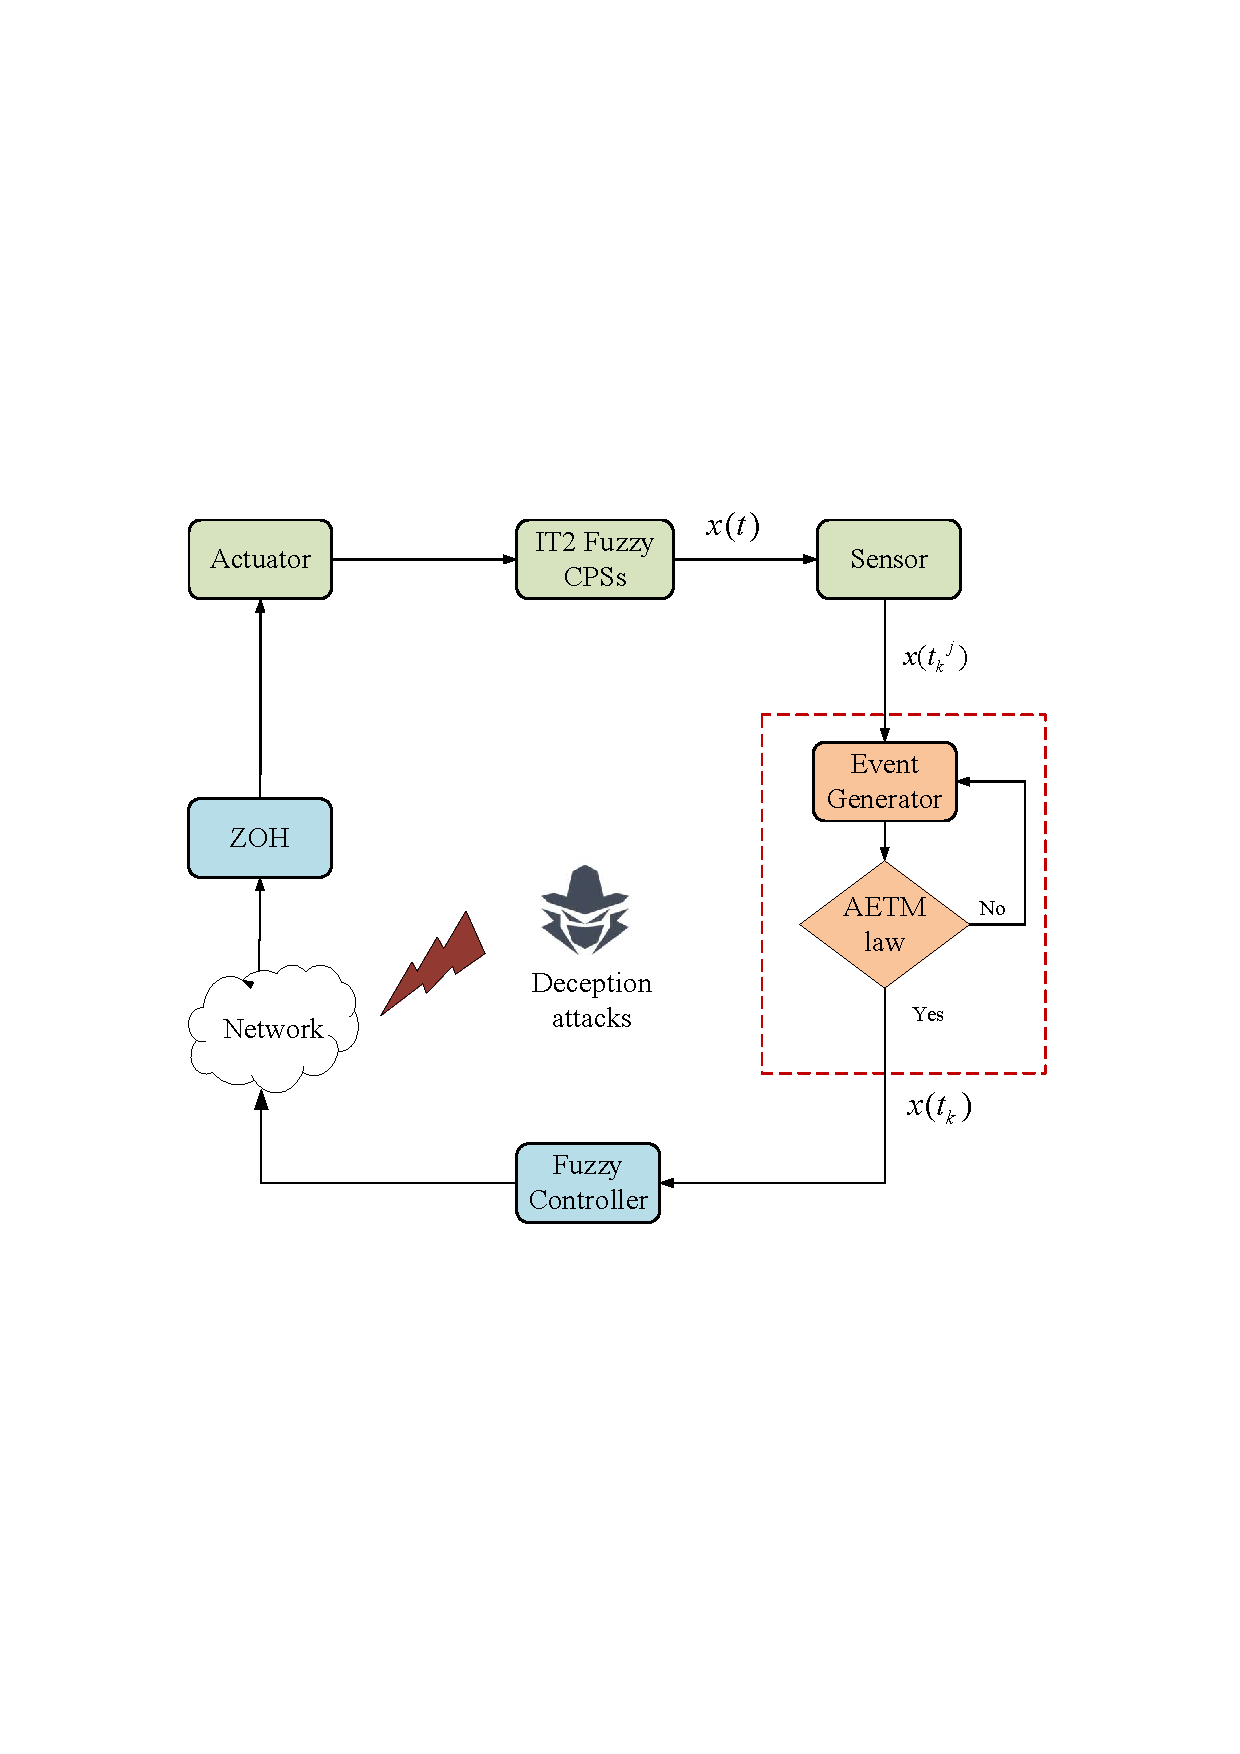
\includegraphics[width=4in]{figs/system_big.pdf} 
	\caption{Architecture of the IT-2 fuzzy CPSs under deception attacks and actuator failures.}
	\label{fig1}
\end{figure}

\subsection{Adaptive Event-Triggered Mechanism}\label{sec2.2}
In networked control systems (NCSs), continuous data transmission often leads to network congestion and unnecessary waste of limited communication bandwidth. To alleviate the communication burden while preserving the desired control performance and avoiding unnecessary transmissions, an AETM is deployed along the sensor-to-controller communication path.

Specifically, the sensor periodically samples the system state with a sampling period $h>0$. Let $t_kh$ ($k \in \mathbb{N}$, $t_0 = 0$) denote the $k$-th successful transmission instant. Under a zero-order hold (ZOH) scheme, the transmitted state $x(t_k h)$ remains unchanged before the subsequent triggering instant $t_{k+1}h$, which is specified as follows:
\begin{equation} \label{eq:Event_TR_1}
	t_{k+1}h = t_k h + \inf \left\{ jh \mid e^{\mathrm{T}}(t^j_{k}) S e(t^j_{k}) - \delta(t) x^{\mathrm{T}}(t_{k}^j) S x(t_{k}^j) > 0 \right\}
\end{equation}
where $t_k^j=t_kh+jh$ represents the current sampling candidate.
Define the sampling error as
$e(t_k^j)\triangleq x(t_k^j)-x(t_kh)$, which measures the discrepancy between the current sample and the most recently transmitted state.
Here, $S>0$ is a prescribed weighting matrix.

Unlike the traditional static event-triggered scheme with a constant threshold, the parameter $\delta(t)$ is dynamically adjusted to respond to system fluctuations. Specifically, the threshold $\delta(t)$ evolves according to the adaptive differential equation below:
\begin{equation} \label{eq:adaptive_law}
	\dot{\delta}(t) = \frac{1}{\delta(t)} \left( \frac{1}{\delta(t)} - \sigma \right) e^{\mathrm{T}}(t^j_{k}) S e(t^j_{k})
\end{equation}
with a given initial condition $\delta(0) \in (0, 1]$. Here, $\sigma>0$ governs the convergence speed of $\delta(t)$.

\begin{rem}
	According to the adaptive law \eqref{eq:adaptive_law}, the adjustment direction of $\delta(t)$ is determined by the term $1/\delta(t)-\sigma$, while the magnitude of the adjustment is scaled by the triggering error $e(t^j_k)$. Thus, the parameter $\delta(t)$ is driven toward the equilibrium value $1/\sigma$ when the triggering error is nonzero. A larger error accelerates this adaptive process, enabling the event-triggering threshold to respond to variations caused by disturbances or cyberattacks. When the triggering error is small, the update of $\delta(t)$ is weakened, thereby avoiding unnecessary fluctuations of the threshold and reducing redundant data transmissions.
\end{rem}

\subsection{Characterization of Deception Attacks}\label{sec2.3}
In NCSs, transmitted signals may be corrupted due to malicious interference in communication channels. In particular, deception attacks can inject falsified data into the transmission process, which may distort the original information and severely degrade system performance.

To characterize the occurrence of deception attacks, let $\theta(t)$ denote a Bernoulli random variable taking values in $\{0,1\}$, where $\theta(t)=1$ indicates that the transmitted data is compromised by the attacker, and $\theta(t) = 0$ otherwise. Such a Bernoulli process is commonly employed to describe randomly occurring deception attacks in networked control systems. It is assumed that $\theta(t)$ satisfies the following statistical property:
\begin{equation}
	\mathbb{E}\{\theta(t)\} = \bar{\theta} 
\end{equation}
where $\bar{\theta} \in [0,1]$ represents the probability of a deception attack.
The stochastic process $\theta(t)$ is assumed to be independent of the system state, actuator failure mode, and external disturbance.

Consequently, under the considered attack model, the signal $x_c(t)$ received by the controller is expressed as:
\begin{equation}\label{eq:deception_attacks}
	x_c(t_{k} h) = (1 - \theta(t_{k} h)) x(t_{k} h) + \theta(t_{k} h) f(x(t_{k} h))
\end{equation}
where $f(x(t_{k}h)) \in \mathbb{R}^{n_x}$ represents the nonlinear deception signal injected by the adversary to replace the original state information.

\begin{asptn} \label{assump:attack_bound}
The nonlinear deception signal $f(x(t))$ is assumed to satisfy
\begin{equation}
	|f_k(x(t))| \le L_k |x_k(t)|,\quad k = 1,2,\ldots,n_x
\end{equation}
where $L_k > 0$ denotes a positive constant representing the attack intensity on the $k$-th state component.
\end{asptn}
\begin{rem}
	Different from Denial-of-Service attacks that aim to block communication channels
	and cause packet dropouts, deception attacks maliciously tamper with the transmitted data packets to
	degrade system performance or even destabilize the system. The expression \eqref{eq:deception_attacks} unifies normal data transmission ($\theta(t) = 0$) and successful deception attacks ($\theta(t) = 1$) into
	a single framework. Moreover, the norm-bounded condition in Assumption \ref{assump:attack_bound} is broadly adopted to
	describe practical limitations on the attack intensity, since adversaries cannot inject unbounded signals
	into the communication network.
\end{rem}

\subsection{Controller Design with Actuator Failures}
In this section, an IT-2 fuzzy controller is synthesized. Based on the corrupted and triggered signal $x_c(t_k h)$, the $n$-th controller rule is formulated as:

\textbf{Controller Rule $n$:} 
\textbf{IF} $\phi_1(x(t))$ is $J^{n}_1$ \textbf{and} $\dots$ \textbf{and} $\phi_p(x(t))$ is $J^{n}_p$, \textbf{THEN}
\begin{equation} 
	u(t) = K_{n} x_c(t_{k} h), \quad n = 1, 2, \ldots, r
\end{equation}
where $K_n$ denote the controller gains to be designed. Through fuzzy blending, the resulting control law takes the form
\begin{equation} 
	u(t) = \sum_{n=1}^{r} h_n(x(t)) K_{n} x_c(t_k h).
\end{equation}

To account for stochastic actuator failures, the actual control signal takes the form
\begin{equation}\label{eq:local_controller}
	u(t) = \sum_{n=1}^{r} h_n(x(t)) F_{r(t)} K_{n} x_c(t_k h),
\end{equation}

For notational convenience, let $i = r(t)$. 
Then $F_i = F_{r(t)} \in \mathbb{R}^{n_u \times n_u}$ is defined as $F_i = \operatorname{diag}\{f_{i}^1, f_{i}^2, \ldots, f_{i}^{n_u}\}$, where $0 \le f_{i-}^{k} \le f_{i}^{k} \le f_{i+}^{k} \le 1,\ (k = 1,2,\ldots,n_u)$. $f_{i-}^{k}$ and $f_{i+}^{k}$ are known real constants. 
Defining $\bar{f}_{i}^{k} = \frac{f_{i+}^{k} + f_{i-}^{k}}{2}$ and $\underline{f}_{i}^{k} = \frac{f_{i+}^{k} - f_{i-}^{k}}{2}$, one obtains
\begin{equation}\label{F_i01}
	F_{i}= F_{i0}+F_{i1} V_{i}
\end{equation}
where $F_{i0} = \operatorname{diag}\{\bar{f}_{i}^{1}, \bar{f}_{i}^{2}, \ldots, \bar{f}_{i}^{n_u}\}$, $F_{i1} = \operatorname{diag}\{\underline{f}_{i}^{1}, \underline{f}_{i}^{2}, \ldots, \underline{f}_{i}^{n_u}\}$, $V_i = \operatorname{diag}\{v_{i}^{1}, v_{i}^{2}, \ldots, v_{i}^{n_u}\}$ for $v_i^k \in [-1,1]$. Then, $V_i^\mathrm{T}V_i \le I$ holds.

The stochastic parameter $r(t)$ evolves as a right-continuous Markov chain over the finite state set $\mathbb{J} \triangleq \{1,2,\dots,J\}$. The corresponding transition-rate matrix $\Pi \triangleq [\lambda_{ij}] \in \mathbb{R}^{J \times J}$ is characterized by
\begin{equation} \label{eq:markov_jump}
	\Pr\{r(t+\Delta t) = j \mid r(t) = i\}
	=
	\begin{cases}
		\lambda_{ij}\Delta t + o(\Delta t), & i \neq j \\
		1 + \lambda_{ii}\Delta t + o(\Delta t), & i = j
	\end{cases}
\end{equation}
where $\Delta t > 0$ and $\lim_{\Delta t \to 0} (o(\Delta t) / \Delta t) = 0$. For any $i, j \in \mathbb{J}$, the transition rates $\lambda_{ij}$ satisfy $\lambda_{ij} \ge 0$ for $i \neq j$, and $\lambda_{ii} = -\sum_{j \in \mathbb{J}, j \neq i} \lambda_{ij}$.

By substituting the controller \eqref{eq:local_controller} into the system \eqref{eq:global_system}, and considering the stochastic deception attack model \eqref{eq:deception_attacks}, the closed-loop system for $t \in [t_k h + jh, t_k h + (j+1)h)$ is formulated as:
\begin{equation} \label{eq:closed_loop}
	\left\{
	\begin{aligned}
		\dot{x}(t) &= \sum_{m=1}^{r} \sum_{n=1}^{r} h_m h_n \Big\{ A_{m} x(t) + B_{m} F_{i} K_{n} \big[ (1-\theta(t_k h)) x(t_k h) + \theta(t_k h) f(x(t_k h)) \big] + E_{m} w(t) \Big\} \\
		z(t) &= \sum_{m=1}^{r} \sum_{n=1}^{r} h_m h_n C x(t) 
	\end{aligned}
	\right.
\end{equation}
where $h_m$ and $h_n$ denote $h_m(x(t))$ and $h_n(x(t))$, respectively.

\begin{Lem} (\cite{wangNewApproachStability2018})
\label{lem:MFD_derivative}
For $G_h=\sum_{m=1}^r h_mG_m$, the inequality $\dot G_h\le0$ is guaranteed whenever the following conditions hold:
	\begin{equation} \label{eq:switching_logic_base}
		\begin{cases}
			\text{if } \dot{h}_v \leq 0, \text{ then } & G_{v} - G_{r} \ge 0, \\
			\text{if } \dot{h}_v > 0, \text{ then } & G_{v} - G_{r} \leq 0,
		\end{cases}
	\end{equation}
	where $v = 1, \dots, r-1$.
\end{Lem}

\begin{rem} \label{rem:Vl_definition}
	Lemma \ref{lem:MFD_derivative} indicates that the state space can be partitioned into $2^{r-1}$ operational regions, denoted by $\mathcal{V}_l$ ($l = 1,2,\dots,2^{r-1}$), according to the sign combinations of $\dot{h}_v$. Correspondingly, each region $\mathcal{V}_l$ is associated with a set of matrix inequalities, denoted by $\mathcal{C}_l$, which are derived from the switching conditions in \eqref{eq:switching_logic_base}. Here, the $r$-th rule is selected as the reference rule for constructing the matrix conditions.
\end{rem}

Motivated by Lemma \ref{lem:MFD_derivative}, a corresponding piecewise control strategy is designed. Based on the switching information characterized by the sign of $\dot h_v$, the controller gains are designed to be region-dependent. Consequently, the piecewise fuzzy controller \eqref{eq:local_controller} is reformulated as follows:
\begin{equation} \label{eq:switching_controller}
	u(t) =
	\begin{cases}
		\sum_{n=1}^{r} h_n F_i K_{n}^1 x_c(t_k h), & x(t)\in \mathcal{V}_1, \\
		\vdots & \vdots \\
		\sum_{n=1}^{r} h_n F_i K_{n}^l x_c(t_k h), & x(t)\in \mathcal{V}_l.
	\end{cases}
\end{equation}

Corresponding to the switching fuzzy controller, the adaptive event-triggering condition \eqref{eq:Event_TR_1} is evaluated within each operational region. Specifically, the triggering mechanism is formulated as
\begin{equation} 
 e^{\mathrm{T}}(t^j_{k}) S^l e(t^j_{k}) - \delta(t) x^{\mathrm{T}}(t_{k}^j) S^l x(t_{k}^j) > 0, \quad \text{for } \mathcal{V}_l
\end{equation}
where $S^l>0$ denotes the event-triggering weight matrix associated with the operational region $\mathcal{V}_l$, and the specific switching conditions for each $\mathcal{V}_l$ are defined according to Lemma \ref{lem:MFD_derivative}.

\begin{Lem}\label{lem2}(\cite{guanModifiedLoopedFunctional2021a}) 
Consider a symmetric positive definite matrix $R \in \mathbb{R}^{n\times n}$, a vector $\zeta \in \mathbb{R}^{m}$, and free-weighting matrices $Y_1, Y_2 \in \mathbb{R}^{n\times m}$. For every continuously differentiable function $x : [a,b] \rightarrow \mathbb{R}^{n}$, the following inequality holds:
\begin{align}
	-\int_{a}^{b} \dot{x}^{\mathrm{T}}(\eta) R \dot{x}(\eta) \mathrm{d}\eta 
	\le & \ (b-a) \zeta^{\mathrm{T}} \left[ Y_1^{\mathrm{T}} R^{-1} Y_1 
	+ \frac{(b-a)^2}{3} Y_2^{\mathrm{T}} R^{-1} Y_2 \right] \zeta 
	 + 2\zeta^{\mathrm{T}} \left[ Y_1^{\mathrm{T}} (x(b) - x(a)) 
	 - 2Y_2^{\mathrm{T}} \int_{a}^{b} x(\eta)\mathrm{d}\eta \right] \notag \\
	& + 2(b-a) \zeta^{\mathrm{T}} Y_2^{\mathrm{T}} (x(b) + x(a)).
\end{align}
\end{Lem} 

\begin{Def}\label{Def1}
	The closed-loop IT-2 fuzzy CPS in \eqref{eq:closed_loop} is asymptotically stable with an $\mathrm{H}_\infty$ performance level $\gamma>0$ if the following two requirements are fulfilled:
	
	\begin{enumerate}
		\item In the absence of external disturbance, i.e., $w(t)=0$, the resultant IT-2 fuzzy CPSs \eqref{eq:closed_loop} is asymptotically stable.
		
		\item For zero initial conditions and every nonzero disturbance input $w(t)\in L_2[0,+\infty)$, the inequality below is satisfied:
		\begin{equation}
			\int_0^{+\infty}
			\mathbb E\left\{
			z^\mathrm{T}(t)z(t)
			\right\}dt
			\le
			\gamma^2
			\int_0^{+\infty}
			\mathbb E\left\{
			w^\mathrm{T}(t)w(t)
			\right\}dt
		\end{equation}
	\end{enumerate}
	where $\gamma>0$ stands for the prescribed level of disturbance‑attenuation performance.

\end{Def}

\section{Main Results}\label{sec3}
This section presents the main results. On the basis of the established system model, an appropriate Lyapunov functional is constructed to obtain sufficient criteria guaranteeing the asymptotic stability and prescribed $\mathrm{H}_\infty$ performance of the closed-loop system.

Recall that $t_k^j=t_k h+jh$ denotes the current sampling instant. For compact representation, the following notations are introduced:
\begin{equation*}
	d_1(t) = t - t^j_k, \quad  
	d_2(t) = t^{j+1}_{k} - t.
\end{equation*}
\begin{equation*}
	\zeta_1(t) = \mathrm{col} \left\{ x(t^j_k),  x(t^{j+1}_{k}) \right\}, \quad
	\zeta_2(t) = \mathrm{col} \left\{ x(t), x(t_k^j), \int_{t_k^j}^t x(\eta) d\eta \right\},
\end{equation*}
\begin{equation*}
	\zeta_3(t) = \mathrm{col} \left\{ x(t), x(t_k^{j+1}), \int_t^{t_k^{j+1}} x(\eta) d\eta \right\}.
\end{equation*}
\begin{equation*}
	\varepsilon(t) = \mathrm{col}\left[
	x(t),   \dot{x}(t),   x(t_k h),
	x(t_k^j),   x(t^{j+1}_k),
	\int_{t_k^j}^{t} x(\eta) d\eta,
	\int_{t}^{t_k^{j+1}} x(\eta) d\eta,
	f(x(t_k h)),  w(t)
	\right]
\end{equation*}
\begin{equation*}
	e_l = \left[ 0_{n_x \times (l-1)n_x}, I_{n_x}, 0_{n_x \times ((8-l)n_x+n_w)} \right],\quad l = 1,2,\dots,8,\qquad e_9 = \left[ 0_{n_w \times 8n_x}, I_{n_w} \right].
\end{equation*}
\begin{equation*}
	\Gamma_{1}=\mathrm{col}\{e_{4},e_{5}\},\quad
	\Gamma_{2}=\mathrm{col}\{e_{1},e_{4},e_{6}\},
\end{equation*}
\begin{equation*}
	\Gamma_{3}=\mathrm{col}\{e_{2},0_{n_x\times (8n_x+n_w)},e_{1}\},\quad
	\Gamma_{4}=\mathrm{col}\{e_{1},e_{5},e_{7}\},\quad
	\Gamma_{5}=\mathrm{col}\{e_{2},0_{n_x\times (8n_x+n_w)},-e_{1}\}.
\end{equation*}
\begin{equation*}
	\Gamma_{6}=e_{1} - e_{4},\quad
	\Gamma_{7}=e_{1} + e_{4},\quad
	\Gamma_{8}=e_{5} - e_{1},\quad
	\Gamma_{9}=e_{5} + e_{1},
\end{equation*}
\begin{equation*}
	\Gamma_{10}=e_{4} - e_{3},
	\quad
	\Gamma_{11}=Q_1e_{1}+Q_2e_{2}+Q_3e_{3}.
\end{equation*}
\begin{equation*}
	\Gamma_{12}= 
	-e_{2} + A_me_{1} 
	+ \bar{\theta} B_{m} F_{i} K_{n} e_{8}
	+(1-\bar{\theta})B_{m} F_{i} K_{n} e_{3}
	+E_m e_{9}.
\end{equation*}
\begin{equation*}
	\bar{L}= \max_{k \in \{1,2,\ldots,n_x\}} \{L_k\},
	\quad
	L = \mathrm{diag}\{\bar{L}, \bar{L}, \dots, \bar{L}\}.
\end{equation*}

Throughout this section, the subscript $h$ attached to a rule-dependent matrix denotes its fuzzy-weighted counterpart. For the looped-functional terms, let $H_{\ell h}=\sum_{m=1}^{r}h_mH_{\ell m}$ $(\ell=1,2)$, where each $H_{\ell m}$ is a structured symmetric matrix of the form
\begin{equation}\label{eq:H_structure}
	H_{\ell m}=
	\begin{bmatrix}
		\dfrac{X_{\ell 1m}+X_{\ell 1m}^{\mathrm T}}{2}
		&
		-X_{\ell 1m}+X_{\ell 2m}
		&
		X_{\ell 3m}
		\\[1.2ex]
		*
		&
		-X_{\ell 2m}-X_{\ell 2m}^{\mathrm T}
		+\dfrac{X_{\ell 1m}+X_{\ell 1m}^{\mathrm T}}{2}
		&
		X_{\ell 4m}
		\\[1.2ex]
		*
		&
		*
		&
		\dfrac{X_{\ell 5m}+X_{\ell 5m}^{\mathrm T}}{2}
	\end{bmatrix},
\end{equation}
with free matrices $X_{\ell qm}$ $(q=1,\ldots,5)$ of appropriate dimensions.
\begin{thm}\label{thm1}
For given scalars $h>0$, $\bar{\theta}\in[0,1]$, $\sigma>0$, and $\gamma>0$, the closed-loop IT-2 fuzzy CPSs \eqref{eq:closed_loop} is asymptotically stable with a prescribed $\mathrm{H}_\infty$ performance level $\gamma$ if there exist symmetric positive definite matrices
$P_{im}$, $M_m$, $R_{1m}$, $R_{2m}$, $S$, a diagonal positive definite matrix $\Lambda$,
structured symmetric matrices $H_{1m}$ and $H_{2m}$ in the form of \eqref{eq:H_structure},
and free-weighting matrices
$Y_{11}$, $Y_{12}$, $Y_{21}$, $Y_{22}$, $Q_1$, $Q_2$, and $Q_3$
of appropriate dimensions, such that the following LMIs are feasible for each Markov state $i\in\mathbb{J}$, all $m,n\in\{1,2,\ldots,r\}$, and each operational region $\mathcal V_l$ ($l=1,2,\ldots,2^{r-1}$).
\begin{equation}\label{shucr1}
	\begin{cases}
		\Psi_{gmn} < 0 ,\quad  m=n  \\
		\Psi_{gmn} + \Psi_{gnm} < 0,\quad 1 \le m < n \le r
	\end{cases}
\end{equation}
for $g=1,2$, and
\begin{equation}\label{dot_small_0}
	\dot{P}_{ih} \leq 0, \, 
	\dot{M}_{h} \leq 0, \, 
	\dot{R}_{1h} \leq 0, \, 
	\dot{R}_{2h} \geq 0, \, 
	\dot{H}_{1h} \leq 0, \, 
	\dot{H}_{2h} \leq 0
\end{equation}
where
\begin{equation}\label{LMI1}
	\Psi_{1mn} =
	\begin{bmatrix}
		\Omega_{1mn} & \sqrt{h}Y_{11}^{\mathrm{T}} & \sqrt{h}Y_{12}^{\mathrm{T}} & e_1^{\mathrm{T}} C^{\mathrm{T}} \\[1.5ex]
		* & -R_{1m} & 0 & 0  \\[1.5ex]
		* & * & -\dfrac{3R_{1m}}{h^2} & 0 \\[1.5ex]
		* & * & * & -I
	\end{bmatrix}
\end{equation}
\begin{equation}\label{LMI2}
	\Psi_{2mn} =
	\begin{bmatrix}
		\Omega_{2mn} & \sqrt{h}Y_{21}^{\mathrm{T}} & \sqrt{h}Y_{22}^{\mathrm{T}} & e_1^{\mathrm{T}} C^{\mathrm{T}} \\[1.5ex]
		* & -R_{2m} & 0 & 0 \\[1.5ex]
		* & * & -\dfrac{3R_{2m}}{h^2} & 0  \\[1.5ex]
		* & * & * & -I 

	\end{bmatrix}
\end{equation}
with
\begin{align*}
\Omega_{0mn}
&= \mathrm{Sym}\{e_1^{\mathrm{T}}P_{im}e_2\}
+e_1^{\mathrm{T}}\sum_{j=1}^{J}\lambda_{ij}P_{jm}e_1
-\Gamma_2^{\mathrm{T}}H_{1m}\Gamma_2
+\Gamma_4^{\mathrm{T}}H_{2m}\Gamma_4
 +e_4^{\mathrm{T}}S^le_4
-\sigma\Gamma_{10}^{\mathrm{T}}S^l\Gamma_{10}
+\mathrm{Sym}\{Y_{11}^{\mathrm{T}}\Gamma_6-2Y_{12}^{\mathrm{T}}e_6\}
\\
&\quad
+\mathrm{Sym}\{Y_{21}^{\mathrm{T}}\Gamma_8-2Y_{22}^{\mathrm{T}}e_7\}
+\mathrm{Sym}\{\Gamma_{11}^{\mathrm{T}}\Gamma_{12}\}
-e_8^{\mathrm{T}}\Lambda e_8
+e_3^{\mathrm{T}}L^{\mathrm{T}}\Lambda Le_3
-\gamma^2e_9^{\mathrm{T}}e_9 .
\end{align*}
\begin{align*}
	\Omega_{1mn} =   \Omega_{0mn}
	-h \Gamma_{1}^{\mathrm{T}}{M}_{m}
	\Gamma_{1}
	+ h e_{2}^{\mathrm{T}} R_{2m} e_{2}
	+  \mathrm{Sym} \left\{ 
	h\Gamma_{4}^{\mathrm{T}} H_{2m} \Gamma_{5} \right\}
	+h \mathrm{Sym} \left\{ 
	Y_{12}^{\mathrm{T}}\Gamma_{7}
	\right\}
\end{align*}
\begin{align*}
	\Omega_{2mn} = \Omega_{0mn} 
	+h \Gamma_{1}^{\mathrm{T}}{M}_{m}
	\Gamma_{1}
	+he_{2}^{\mathrm{T}} R_{1m} e_{2}
	+\mathrm{Sym} \left\{ 
	h\Gamma_{2}^{\mathrm{T}} H_{1m} \Gamma_{3} \right\}
	+h \mathrm{Sym} \left\{ 
	Y_{22}^{\mathrm{T}}\Gamma_{9}
	\right\}
\end{align*}
	
\begin{proof} 
	We construct the following Lyapunov functional for stability analysis:
	\begin{align}\label{V}
		V(t) =\sum_{p=1}^{5} V_p(t)
	\end{align}
	where 
	\begin{align}
		V_1(t) = x^{\mathrm{T}}(t)P_{ih}x(t)
	\end{align}
	\begin{align}
		V_2(t) = d_1(t) d_2(t)
		\zeta_1^{\mathrm{T}}(t)
		M_{h} \zeta_1(t)
	\end{align}
	\begin{align}
		V_3(t) = 
		d_2(t) \int_{t_k^j}^{t} \dot{x}^\mathrm{T}(\eta) R_{1h} \dot{x}(\eta) \mathrm{d}\eta 
		- d_1(t) \int_{t}^{t_{k}^{j+1}} \dot{x}^\mathrm{T}(\eta) R_{2h} \dot{x}(\eta) \mathrm{d}\eta
	\end{align}
	\begin{align}
		V_4(t) = d_2(t) \zeta_2^{\mathrm{T}}(t) H_{1h} \zeta_2(t) + d_1(t) \zeta_3^{\mathrm{T}}(t) H_{2h} \zeta_3(t)
	\end{align}
	\begin{align}
		V_5(t) = \frac{1}{2} \delta^2(t)
	\end{align}
	
By examining the structural properties of \eqref{V} and \eqref{eq:H_structure}, one can verify that the synthesized functional maintains strict continuity at the discrete sampling moments. Additionally, the specific components $V_p(t)$ satisfy the looped-functional conditions characteristic of looped functionals, which ensures $V_p(t_k^j) = V_p(t_k^{j+1}) = 0$ for $p \in \{2, 3, 4\}$.

Consequently, along the system trajectories described in \eqref{eq:closed_loop}, the infinitesimal generator $\mathcal{L}$ applied to the Lyapunov function $V(t)$ takes the following form:
\begin{comment}
\begin{align}\label{EV1}
	\mathcal{L}V_1(t) 
	&= 2x^{\mathrm{T}}(t)P_{ih}\dot{x}(t) 
	+ x^{\mathrm{T}}(t)\dot{P}_{ih}x(t) 
	+ x^{\mathrm{T}}(t)\left[ \sum_{j=1}^J \lambda_{ij}P_{jh} \right] x(t) \nonumber \\
	&= \varepsilon^{\mathrm{T}}(t) \left\{ \mathrm{Sym}\{
	e_1^{\mathrm{T}}P_{ih}e_2\} + e_1^{\mathrm{T}}\dot{P}_{ih}e_1 
	+ e_1^{\mathrm{T}} \sum_{j=1}^J \lambda_{ij}P_{jh}e_1 \right\} \varepsilon(t).
\end{align}
\end{comment}
\begin{align}\label{EV1}
	\mathbb{E} \left\{ \mathcal{L}V_{1}(t) \right\}
	&= 2x^{\mathrm{T}}(t)P_{ih}\dot{x}(t) 
	+ x^{\mathrm{T}}(t)\dot{P}_{ih}x(t) 
	+ x^{\mathrm{T}}(t) \big( \sum_{j=1}^J \lambda_{ij}P_{jh} \big) x(t) \nonumber \\
	&= \varepsilon^{\mathrm{T}}(t) \Bigl\{ \mathrm{Sym}\{
	e_1^{\mathrm{T}}P_{ih}e_2\} + e_1^{\mathrm{T}}\dot{P}_{ih}e_1 
	+ e_1^{\mathrm{T}} \sum_{j=1}^J \lambda_{ij}P_{jh}e_1 \Bigl\} \varepsilon(t).
\end{align}
\begin{align}
	\mathbb{E} \left\{ \mathcal{L}V_{2}(t) \right\}
	&= \bigl(d_2(t) - d_1(t)\bigr) \, \zeta_1^{\mathrm{T}}(t) \, M_{h} \, \zeta_1(t) + d_1(t)d_2(t) \, \zeta_1^{\mathrm{T}}(t) \, \dot{M}_{h} \, \zeta_1(t) \nonumber \\
	&= \varepsilon^{\mathrm{T}}(t)
	\Bigl\{ d_2(t)\,\Gamma_{1}^{\mathrm{T}} M_{h} \Gamma_{1}
	- d_1(t)\,\Gamma_{1}^{\mathrm{T}} M_{h} \Gamma_{1} \Bigr\} \varepsilon(t)
	+ d_1(t)d_2(t) \, \zeta_1^{\mathrm{T}}(t) \, \dot{M}_{h} \, \zeta_1(t).
\end{align}
\begin{align}
	 \mathbb{E} \left\{ \mathcal{L}V_{3}(t) \right\} 
	&= - \int_{t_k^j}^{t} \dot{x}^\mathrm{T}(\eta) R_{1h} \dot{x}(\eta) \,\mathrm{d}\eta 
	+ d_2(t) \dot{x}^\mathrm{T}(t) R_{1h} \dot{x}(t)
	+ d_2(t)\int_{t_k^j}^{t} \dot{x}^\mathrm{T}(\eta)\,\dot{R}_{1h}\,\dot{x}(\eta)\,\mathrm{d}\eta \nonumber \\
	&\quad -\int_{t}^{t_{k}^{j+1}} \dot{x}^\mathrm{T}(\eta) R_{2h} \dot{x}(\eta) \,\mathrm{d}\eta
	+ d_1(t) \dot{x}^\mathrm{T}(t) R_{2h}\dot{x}(t)
	- d_1(t)\int_{t}^{t_k^{j+1}} \dot{x}^\mathrm{T}(\eta)\,\dot{R}_{2h}\,\dot{x}(\eta)\,\mathrm{d}\eta \nonumber \\
	&= \varepsilon^\mathrm{T}(t) 
	\Bigl\{ d_2(t)\, e_{2}^\mathrm{T} R_{1h} e_{2} 
	+ d_1(t)\, e_{2}^\mathrm{T} R_{2h} e_{2} \Bigr\} \varepsilon(t)  -\int_{t_k^j}^{t} \dot{x}^\mathrm{T}(\eta) R_{1h} \dot{x}(\eta) \,\mathrm{d}\eta
	-\int_{t}^{t_{k}^{j+1}} \dot{x}^\mathrm{T}(\eta) R_{2h} \dot{x}(\eta) \,\mathrm{d}\eta \nonumber \\
	&\quad + d_2(t)\int_{t_k^j}^{t} \dot{x}^\mathrm{T}(\eta)\,\dot{R}_{1h}\,\dot{x}(\eta)\,\mathrm{d}\eta
	- d_1(t)\int_{t}^{t_k^{j+1}} \dot{x}^\mathrm{T}(\eta)\,\dot{R}_{2h}\,\dot{x}(\eta)\,\mathrm{d}\eta .
\end{align}
\begin{align}
	\mathbb{E} \left\{ \mathcal{L}V_{4}(t) \right\} 
	&= -\zeta_2^{\mathrm{T}}(t) H_{1h} \zeta_2(t) + \zeta_3^{\mathrm{T}}(t) H_{2h} \zeta_3(t) + d_2(t) \left( 2\zeta_2^{\mathrm{T}}(t) H_{1h} \dot{\zeta}_2(t) + \zeta_2^{\mathrm{T}}(t) \dot{H}_{1h} \zeta_2(t) \right) \nonumber \\
	&\quad + d_1(t) \left( 2\zeta_3^{\mathrm{T}}(t) H_{2h} \dot{\zeta}_3(t) + \zeta_3^{\mathrm{T}}(t) \dot{H}_{2h} \zeta_3(t) \right) \nonumber \\
	&= \varepsilon^{\mathrm{T}}(t) 
	\Bigl\{ -\Gamma_{2}^{\mathrm{T}} H_{1h} \Gamma_{2}
	+ \Gamma_{4}^{\mathrm{T}} H_{2h} \Gamma_{4}
	+ 2d_2(t) \Gamma_{2}^{\mathrm{T}} H_{1h} \Gamma_{3}
	+ 2d_1(t) \Gamma_{4}^{\mathrm{T}} H_{2h} \Gamma_{5} \Bigr\} \varepsilon(t) \nonumber \\
	&\quad + d_2(t) \zeta_2^{\mathrm{T}}(t) \dot{H}_{1h} \zeta_2(t)
	+ d_{1}(t) \zeta_3^{\mathrm{T}}(t) \dot{H}_{2h} \zeta_3(t).
\end{align}

According to \eqref{eq:Event_TR_1} and \eqref{eq:adaptive_law}, one obtains:
\begin{align}
	\mathbb{E} \left\{ \mathcal{L}V_{5}(t) \right\}
	 = 
	\dot{\delta}(t) \delta(t)
	=\left( \frac{1}{\delta(t)} - \sigma \right) e^{\mathrm{T}}(t^j_{k}) S e(t^j_{k})
	\leq \varepsilon^{\mathrm{T}}(t) 
	\left\lbrace 
	e_{4}^{\mathrm{T}} S e_{4}  
	-\sigma \Gamma_{10}^{\mathrm{T}} S \Gamma_{10}
	\right\rbrace 
	 \varepsilon(t)
\end{align}

Applying Lemma \ref{lem2} to the integral terms yields the following inequalities: 
\begin{align}
	-\int_{t_k^j}^{t} \dot{x}^{\mathrm{T}}(\eta) R_{1h} \dot{x}(\eta) \mathrm{d}\eta 
	\le & \ \varepsilon^{\mathrm{T}}(t) \left[ 
	d_1(t) \left( 
	Y_{11}^{\mathrm{T}} R_{1h}^{-1} Y_{11} 
	+ \frac{h^2}{3} Y_{12}^{\mathrm{T}} R_{1h}^{-1} Y_{12} 
	\right) 
	+ \mathrm{Sym} \left\{ Y_{11}^{\mathrm{T}}\Gamma_{6}  -2Y_{12}^{\mathrm{T}}e_6 
	+d_1(t)Y_{12}^{\mathrm{T}}\Gamma_{7} \right\} \right] \varepsilon(t). \label{eq:bound1}
\end{align}

\begin{align}
	-\int_{t}^{t_k^{j+1}} \dot{x}^{\mathrm{T}}(\eta) R_{2h} \dot{x}(\eta) \mathrm{d}\eta 
	\le & \ \varepsilon^{\mathrm{T}}(t) \left[ 
	d_2(t) \left( 
	Y_{21}^{\mathrm{T}} R_{2h}^{-1} Y_{21} 
	+ \frac{h^2}{3} Y_{22}^{\mathrm{T}} R_{2h}^{-1} Y_{22} \right)  
	 + \mathrm{Sym} \left\{ Y_{21}^{\mathrm{T}}\Gamma_{8} - 2Y_{22}^{\mathrm{T}}e_7 
	+ d_2(t)Y_{22}^{\mathrm{T}}\Gamma_{9} \right\} \right] \varepsilon(t). \label{eq:bound2}
\end{align}

Moreover, in view of the deception-attack characteristics, Assumption \ref{assump:attack_bound} implies that, for any positive diagonal matrix $\Lambda$, the following relation holds:
\begin{equation}\label{eq:normal_decept}
	f^{\mathrm{T}}(x(t_k h)) \Lambda f(x(t_k h)) \le x^{\mathrm{T}}(t_k h) L^{\mathrm{T}} \Lambda L x(t_k h).
\end{equation}

Using the augmented vector $\varepsilon(t)$ defined above, inequality \eqref{eq:normal_decept} takes the following form:
\begin{equation} \label{eq:epsilon_attack_bound}
	\varepsilon^{\mathrm{T}}(t)
	\left\lbrace 
	e_{8}^{\mathrm{T}}  \Lambda e_{8} 
	-e_{3}^{\mathrm{T}} L^{\mathrm{T}}  \Lambda  L e_{3} 
	\right\rbrace 
	\varepsilon(t) \leq 0.
\end{equation}

Additionally, considering the closed-loop IT-2 fuzzy CPSs \eqref{eq:closed_loop}, the following identity holds for any matrices $Q_1$, $Q_2$ and $Q_3$ of appropriate dimensions:
\begin{equation} \label{eq:Zero}
\begin{aligned}
	2 & 
	\sum_{m=1}^{r} \sum_{n=1}^{r} h_m h_n
	\mathbb{E} \biggl\{ \bigl[ x^\mathrm{T}(t) {Q}_1^\mathrm{T} 
	+\dot{x}^\mathrm{T}(t){Q}_2^\mathrm{T}
	+x^\mathrm{T}(t_k h){Q}_3^\mathrm{T}
	\bigr] \\
	& \times \bigl[ 
	-\dot{x}(t) + {A}_{m} x(t) 
	+ B_{m} F_{i} K_{n} \bigl( (1-\theta(t_k h)) x(t_k h) + \theta(t_k h) f(x(t_k h)) \bigr)
	+ E_{m} w(t) \bigr] \biggr\} = 0.
\end{aligned}
\end{equation}

Using the augmented vector $\varepsilon(t)$ together with the definitions of $\Gamma_{11}$ and $\Gamma_{12}$, \eqref{eq:Zero} can be expressed as
\begin{equation} \label{eq:compact_VEQ}
	\sum_{m=1}^{r} \sum_{n=1}^{r} h_m h_n
	\mathbb{E} \left\lbrace 
	\varepsilon^{\mathrm{T}}(t) 
	\left\lbrace 
	\mathrm{Sym} \left\{ 
	\Gamma_{11}^{\mathrm{T}} \Gamma_{12}
	\right\} 
	\right\rbrace 
	\varepsilon(t)
	\right\rbrace 
	= 0.
\end{equation}

By virtue of $\sum_{m=1}^{r}\dot{h}_m=0$, the derivative of the MF-dependent terms takes the following form:
\begin{equation}
\dot{P}_{ih} = \sum_{m=1}^{r} \dot{h}_m P_{im} = \sum_{v=1}^{r-1} \dot{h}_v (P_{iv} - P_{ir})
\end{equation}
\begin{equation}
	\dot{M}_{h} = \sum_{m=1}^{r} \dot{h}_m M_{m} = \sum_{v=1}^{r-1} \dot{h}_v (M_{v} - M_{r})
\end{equation}
\begin{equation}
	\dot{R}_{kh} = \sum_{m=1}^{r} \dot{h}_m R_{km} = \sum_{v=1}^{r-1} \dot{h}_v (R_{kv} - R_{kr})
\end{equation}
\begin{equation}
	\dot{H}_{kh} = \sum_{m=1}^{r} \dot{h}_m H_{km} = \sum_{v=1}^{r-1} \dot{h}_v (H_{kv} - H_{kr})
\end{equation}
where $k = 1, 2$, and $\dot{h}_v$ denotes the time derivative of the $v$-th membership function, whose sign may vary during system operation. According to the sign of $\dot{h}_v$, corresponding matrix inequality constraints are imposed to guarantee the desired inequalities of the MF-dependent matrix derivatives, including $\dot P_{ih}$, $\dot M_h$, $\dot R_{kh}$, and $\dot H_{kh}$. Based on Lemma \ref{lem:MFD_derivative}, the sign-dependent constraints for each $v=1,\ldots,r-1$ are specified as follows:
\begin{equation}
	\begin{cases}
		\textbf{If } \dot{h}_v \le 0,\ \textbf{Then } \mathcal{C}_1, \\[6pt]
		\textbf{If } \dot{h}_v > 0,\ \textbf{Then } \mathcal{C}_2.
	\end{cases}
\end{equation}
where 
\begin{align*}
	\mathcal{C}_1=\{P_{iv}-P_{ir} \ge 0, M_{v}-M_{r} \ge 0, 
	R_{1v}-R_{1r} \ge 0,
	R_{2v}-R_{2r} \leq 0,
	H_{1v}-H_{1r} \ge 0, 
	H_{2v}-H_{2r} \ge  0\},
\end{align*}
\begin{align*}
	\mathcal{C}_2=\{P_{iv}-P_{ir} \le 0, M_{v}-M_{r} \le 0, 
	R_{1v}-R_{1r} \le 0, 
	R_{2v}-R_{2r} \ge 0, 
	H_{1v}-H_{1r} \le 0, 
	H_{2v}-H_{2r} \le 0\}.
\end{align*}

Notice that the sign variations of $\dot{h}_v$ generate $2^{r-1}$ distinct operational modes. Let the set $\mathcal{V}_l$ characterize the $l$-th specific sign combination of the membership function derivatives, and let $\mathcal{C}_l$ collect the corresponding constraints for all $v=1,\ldots,r-1$. Consequently, the switching mechanism can be mathematically formalized by the following logical implication:
\begin{equation}
	\text{If } \mathcal{V}_l, \text{ then } \mathcal{C}_l. \label{eq_if_then_2}
\end{equation}

Combining the preceding derivative estimates, integral inequalities, deception-attack bound, and switching constraints, the following result can be deduced for any $i \in \mathbb{J}$ within the time interval $t \in [t_k^j, t_k^{j+1})$:
\begin{align}
	\mathbb{E}\{\mathcal{L}V(t)\}
	&\leq
	\sum_{m=1}^{r} \sum_{n=1}^{r} h_m h_n \varepsilon^\mathrm{T}(t) \Bigg( 
	\frac{t - t_k^j}{h} \bigg( 
	\Omega_{1mn} 
	+ h  Y_{11}^{\mathrm{T}} R_{1m}^{-1} Y_{11} 
	+ \frac{h^3}{3} Y_{12}^{\mathrm{T}} R_{1m}^{-1} Y_{12}
	+ e_{1}^{\mathrm{T}} C^{\mathrm{T}}C e_1 \bigg) \notag \\
	&\quad + \frac{t_{k}^{j+1} - t}{h} \bigg( 
	\Omega_{2mn} 
	+ h Y_{21}^{\mathrm{T}} R_{2m}^{-1} Y_{21} 
	+ \frac{h^3}{3} Y_{22}^{\mathrm{T}} R_{2m}^{-1} Y_{22}
	+ e_{1}^{\mathrm{T}} C^{\mathrm{T}}C e_1  
	\bigg) \Bigg) \varepsilon(t) 
	- z^{\mathrm{T}}(t)z(t) + \gamma^2 w^{\mathrm{T}}(t)w(t).
\end{align}
\begin{comment}
	\begin{align}
		\mathbb{E}\{\mathcal{L}V(t)\}
		&\leq
		\mathbb{E} \Bigg\{
		\sum_{m=1}^{r} \sum_{n=1}^{r} h_m h_n \varepsilon^\mathrm{T}(t) \Bigg( 
		\frac{t - t_k^j}{h} \bigg( 
		\Omega_{1mn} 
		+ h  Y_{11}^{\mathrm{T}} R_{1m}^{-1} Y_{11} 
		+ \frac{h^3}{3} Y_{12}^{\mathrm{T}} R_{1m}^{-1} Y_{12}
		+ e_{1}^{\mathrm{T}} C^{\mathrm{T}}C e_1 \bigg) \notag \\
		&\quad + \frac{t_{k}^{j+1} - t}{h} \bigg( 
		\Omega_{2mn} 
		+ h Y_{21}^{\mathrm{T}} R_{2m}^{-1} Y_{21} 
		+ \frac{h^3}{3} Y_{22}^{\mathrm{T}} R_{2m}^{-1} Y_{22}
		+ e_{1}^{\mathrm{T}} C^{\mathrm{T}}C e_1  
		\bigg) \Bigg) \varepsilon(t) 
		- z^{\mathrm{T}}(t)z(t) + \gamma^2 w^{\mathrm{T}}(t)w(t)
		\Bigg\}.
	\end{align}
\end{comment}

Based on the Schur complement, condition \eqref{shucr1} guarantee the negativity of the corresponding fuzzy-weighted double-sum terms. By exploiting the convex combination property of the membership functions, i.e., $h_m \ge 0$ and $\sum_{m=1}^{r} h_m = 1$, one can obtain
\begin{equation}
	\mathbb{E}\{\mathcal{L}V(t)\}
	\leq
	\mathbb{E} \left\{
	-z^{\mathrm{T}}(t)z(t)
	+\gamma^2 w^{\mathrm{T}}(t)w(t)
	\right\}.
\end{equation}

\textbf{Case \uppercase\expandafter{\romannumeral1}:} When $w(t)=0$, it follows that
\begin{equation}
	\mathbb{E}\{\mathcal{L}V(t)\}
	\leq
	-\mathbb{E}\{z^{\mathrm{T}}(t)z(t)\}
	\leq 0.
\end{equation}

Thus, the closed-loop IT-2 fuzzy CPSs \eqref{eq:closed_loop} is asymptotically stable.

\textbf{Case \uppercase\expandafter{\romannumeral2}:} When $w(t)\neq0$, integrating both sides over $[0,+\infty)$ yields
\begin{equation}
	\mathbb{E}\left\{V(+\infty)-V(0)\right\}
	\leq
	\int_{0}^{+\infty}
	\mathbb{E}\left\{
	-z^{\mathrm{T}}(t)z(t)
	+\gamma^2 w^{\mathrm{T}}(t)w(t)
	\right\}dt.
\end{equation}

Under the zero initial condition and using $V(+\infty)\ge0$, it follows that
\begin{equation}
	\int_{0}^{+\infty}
	\mathbb{E}\left\{
	z^{\mathrm{T}}(t)z(t)
	\right\}dt
	\leq
	\gamma^2
	\int_{0}^{+\infty}
	\mathbb{E}\left\{
	w^{\mathrm{T}}(t)w(t)
	\right\}dt.
\end{equation}

Therefore, the resultant IT-2 fuzzy CPS \eqref{eq:closed_loop} satisfies $\mathrm{H}_\infty$ performance. The proof is thus finished.
\end{proof}
\end{thm}
\begin{rem}
The construction of the two-sided FMF-dependent looped functional in \eqref{V} is central to the derivation of Theorem~3.1.
By incorporating the augmented vectors $\zeta_i(t)$ $(i=1,2,3)$ and the sampling-interval distances $d_i(t)$ $(i=1,2)$, the looped and integral terms exploit the state information within $[t_k^j,t_k^{j+1})$.
These structural refinements, along with the adaptive threshold $\delta(t)$ and the region-dependent partitioning based on $\dot{h}_v$, help reduce conservatism in Theorem \ref{thm1}.
Furthermore, this methodological framework is not restricted to the current system and can be extended to other networked or sampled-data systems.
\end{rem}
Theorem \ref{thm1} provides stability and prescribed $\mathrm{H}_{\infty}$ performance criteria for the closed-loop system.
However, due to the presence of coupled decision variables, the controller gain matrices cannot be explicitly obtained. Therefore, Theorem \ref{thm2} provides a numerically tractable LMI framework for controller synthesis.
\begin{thm}\label{thm2}
 For given scalars $h > 0$, $\bar{\theta} \in [0,1]$, $\sigma > 0$, $\gamma > 0$, $\xi_1$ and $\xi_2$, the closed-loop IT-2 fuzzy CPSs \eqref{eq:closed_loop} is asymptotically stable with a prescribed $\mathrm{H}_\infty$ performance level $\gamma$ if there exist symmetric positive definite matrices $\tilde{P}_{im}$, $\tilde{M}_{m}$, $\tilde{R}_{1m}$, $\tilde{R}_{2m}$, $\tilde{S}$, $\tilde{\Lambda}$, structured symmetric matrices $\tilde{H}_{1m}$ and $\tilde{H}_{2m}$, a nonsingular matrix $\tilde{N}$, and matrices $\tilde{Y}_{11}$, $\tilde{Y}_{12}$, $\tilde{Y}_{21}$, $\tilde{Y}_{22}$, and $\widetilde{K}_n$ with appropriate dimensions, such that for each Markov state $i \in \mathbb{J}$, fuzzy rules $m,n = 1,2,\ldots,r$, and switching condition $\mathcal{C}_l$ ($l = 1,2,\ldots,2^{r-1}$), the following LMIs are feasible:
	\begin{equation}\label{shucr1_not}
		\begin{cases}
			\widetilde{\Psi}_{gmn} < 0 	,\quad  m=n  \\
			\widetilde{\Psi}_{gmn} + \widetilde{\Psi}_{gnm} < 0,\quad 1 \le m 	< n \le r
		\end{cases}
	\end{equation}
	for $g=1,2$, and
	\begin{equation}\label{dot_hat_small_0}
	\dot{\widetilde{P}}_{ih} \leq 0, \, 
	\dot{\widetilde{M}}_{h} \leq 0, \, 
	\dot{\widetilde{R}}_{1h} \leq 0, \, 
	\dot{\widetilde{R}}_{2h} \geq 0, \, 
	\dot{\widetilde{H}}_{1h} \leq 0, \, 
	\dot{\widetilde{H}}_{2h} \leq 0
	\end{equation}
\begin{equation}\label{LMI1_not}
\widetilde{\Psi}_{1mn} =
\begin{bmatrix}
	\widetilde{\Omega}_{1mn} & \sqrt{h} \widetilde{Y}_{11}^{\mathrm{T}} & \sqrt{h} \widetilde{Y}_{12}^{\mathrm{T}} & e_1^{\mathrm{T}} \widetilde{N}^{\mathrm{T}} {C}^{\mathrm{T}}\\[1.5ex]
	* & -\widetilde{R}_{1m} & 0 & 0 \\[1.5ex]
	* & * & -\dfrac{3\widetilde{R}_{1m}}{h^2} & 0\\[1.5ex]
	* & * & * & -I
\end{bmatrix}
\end{equation}

\begin{equation}\label{LMI2_not}
\widetilde{\Psi}_{2mn} =
\begin{bmatrix}
	\widetilde{\Omega}_{2mn} & \sqrt{h} \widetilde{Y}_{21}^{\mathrm{T}} & \sqrt{h} \widetilde{Y}_{22}^{\mathrm{T}} & e_1^{\mathrm{T}} \widetilde{N}^{\mathrm{T}}C^{\mathrm{T}} \\[1.5ex]
	* & -\widetilde{R}_{2m} & 0 & 0 \\[1.5ex]
	* & * & -\dfrac{3\widetilde{R}_{2m}}{h^2} & 0  \\[1.5ex]
	* & * & * & -I 
\end{bmatrix}
\end{equation}
	with
\begin{align*}
	\widetilde{\Omega}_{0mn} &=  \mathrm{Sym} \{e_1^{\mathrm{T}} \widetilde{P}_{im} e_2\}
	+e_1^{\mathrm{T}}  \sum_{j=1}^J {\lambda}_{ij}\widetilde{P}_{jm} e_1
	-\Gamma_{2}^{\mathrm{T}} \widetilde{H}_{1m} \Gamma_{2}
	+\Gamma_{4}^{\mathrm{T}} \widetilde{H}_{2m} \Gamma_{4}
	+e_{4}^{\mathrm{T}} \widetilde{S} e_{4}
	-\sigma \Gamma_{10}^{\mathrm{T}} \widetilde{S} \Gamma_{10}
	+ \mathrm{Sym} \left\{ \widetilde{Y}_{11}^{\mathrm{T}}\Gamma_{6}  -2\widetilde{Y}_{12}^{\mathrm{T}}e_6
	\right\} \\
	&+\mathrm{Sym} \left\{ \widetilde{Y}_{21}^{\mathrm{T}}\Gamma_{8} - 2\widetilde{Y}_{22}^{\mathrm{T}}e_7  \right\}
	+\mathrm{Sym} \left\{ 
	\widetilde{\Gamma}_{11}^{\mathrm{T}} \widetilde{\Gamma}_{12}
	\right\}
	-e_{8}^{\mathrm{T}}  \widetilde{\Lambda} e_{8} 
	+e_{3}^{\mathrm{T}} L^{\mathrm{T}}  \widetilde{\Lambda}  L e_{3} 
	-\gamma^2 e_{9}^{\mathrm{T}}e_{9}
\end{align*}
\begin{align*}
	\widetilde{\Omega}_{1mn} = &  \widetilde{\Omega}_{0mn}
	-h \Gamma_{1}^{\mathrm{T}}\widetilde{M}_{m}
	\Gamma_{1}
	+ h e_{2}^{\mathrm{T}} \widetilde{R}_{2m} e_{2}
	+h \mathrm{Sym} \left\{
	\Gamma_{4}^{\mathrm{T}} \widetilde{H}_{2m} \Gamma_{5}
	\right\}
	+h \mathrm{Sym} \left\{ 
	\widetilde{Y}_{12}^{\mathrm{T}}\Gamma_{7}
	\right\}
\end{align*}
\begin{align*}
	\widetilde{\Omega}_{2mn} = &\widetilde{\Omega}_{0mn} 
	+h \Gamma_{1}^{\mathrm{T}}\widetilde{M}_{m}
	\Gamma_{1}
	+he_{2}^{\mathrm{T}} \widetilde{R}_{1m} e_{2}
	+h \mathrm{Sym} \left\{
	\Gamma_{2}^{\mathrm{T}} \widetilde{H}_{1m} \Gamma_{3}
	\right\}
	+h \mathrm{Sym} \left\{ 
	\widetilde{Y}_{22}^{\mathrm{T}}\Gamma_{9}
	\right\}
\end{align*}
where $\widetilde{\Gamma}_{11}=e_1+\xi_1e_2+\xi_2e_3$ and
$\widetilde{\Gamma}_{12}
=-\widetilde{N}e_2+A_m\widetilde{N}e_1
+\bar{\theta}B_mF_i\widetilde{K}_ne_8
+(1-\bar{\theta})B_mF_i\widetilde{K}_ne_3+E_me_9$.
In addition, $\Gamma_i$ $(i=1,2,\ldots,10)$, $C$, and $L$ are defined as in Theorem~\ref{thm1}.
Moreover, the controller gain is recovered as
$K_n=\widetilde{K}_n\widetilde{N}^{-1}$.
\begin{proof}
	Define $\widetilde{N}=Q_1^{-1}$, $Q_2=\xi_1 Q_1$ and let $Q_3=\xi_2 Q_1$. Moreover, define
	$\mathcal{N}_2=\mathrm{diag}\{\widetilde{N},\widetilde{N}\}$
	and
	$\mathcal{N}_3=\mathrm{diag}\{\widetilde{N},\widetilde{N},\widetilde{N}\}$. Set $\widetilde{P}_{im}=\widetilde{N}^{\mathrm{T}}P_{im}\widetilde{N}$,
	$\widetilde{M}_m
	=\mathcal{N}_2^{\mathrm{T}}M_m\mathcal{N}_2$,
	$\widetilde{H}_{lm}
	=\mathcal{N}_3^{\mathrm{T}}H_{lm}\mathcal{N}_3$, $\widetilde{R}_{lm}=\widetilde{N}^{\mathrm{T}}R_{lm}\widetilde{N}$, $\widetilde{S}=\widetilde{N}^{\mathrm{T}}S\widetilde{N}$,
	$\widetilde{\Lambda}=\widetilde{N}^{\mathrm{T}}{\Lambda}\widetilde{N}$,
	$\widetilde{Y}_{q1}=\widetilde{N}^{\mathrm{T}}{Y}_{q1}\Sigma_1$,
	$\widetilde{Y}_{q2}=\widetilde{N}^{\mathrm{T}}{Y}_{q2}\Sigma_1$ ($q\in \{1,2\}$)
	and $\widetilde{K}_{n} = K_{n} \widetilde{N}$.
	The congruence matrices are defined as $\Sigma_1 = \mathrm{diag}\{\widetilde{N},\widetilde{N},\widetilde{N},\widetilde{N},\widetilde{N},\widetilde{N},\widetilde{N},\widetilde{N},I_{n_w}\}$. 
	$\Sigma_2 = \mathrm{diag}\{ \Sigma_1,
	\widetilde{N},\widetilde{N},I_{n_z}
	\}$. 
	 By pre- and post-multiplying \eqref{LMI1} and \eqref{LMI2} with $\Sigma_2^{\mathrm{T}}$ and $\Sigma_2$, respectively, the LMIs \eqref{LMI1_not} and \eqref{LMI2_not} are obtained. \eqref{dot_hat_small_0} is derived by applying a congruence transformation to \eqref{dot_small_0}.
\end{proof}
\end{thm}

Notably, the synthesis conditions obtained in Theorem \ref{thm2} still involve the norm-bounded uncertainty matrix $V_i$ caused by stochastic actuator failures. As a result, these conditions cannot be directly solved using standard numerical optimization toolboxes. To overcome this difficulty, Theorem \ref{thm3} introduces a robust bounding technique to eliminate the uncertainty-dependent terms and obtain deterministic LMIs.
\begin{thm}\label{thm3}
	 For given scalars $h>0$, $\bar{\theta}\in[0,1]$, $\sigma>0$, $\gamma>0$, $\xi_1$, $\xi_2$, and $\tau>0$, the closed-loop IT-2 fuzzy system \eqref{eq:closed_loop} is asymptotically stable with a prescribed $\mathrm{H}_\infty$ performance level $\gamma$ if there exist symmetric positive definite matrices 
	$\widetilde{P}_{im}$, 
	$\widetilde{M}_{m}$, 
	$\widetilde{R}_{1m}$, 
	$\widetilde{R}_{2m}$,
	$\widetilde{S}$,
	$\widetilde{\Lambda}$,
	structured symmetric matrices
	$\widetilde{H}_{1m}$ and
	$\widetilde{H}_{2m}$,
	a nonsingular matrix $\widetilde{N}$, 
	and matrices 
	$\widetilde{Y}_{11}$,
	$\widetilde{Y}_{12}$,
	$\widetilde{Y}_{21}$,
	$\widetilde{Y}_{22}$,
	$\widetilde{K}_n$
	with appropriate dimensions, such that for each Markov state $i\in\mathbb{J}$, fuzzy rules $m,n=1,2,\ldots,r$, and switching condition $\mathcal{C}_l$ $(l=1,2,\ldots,2^{r-1})$, the following LMIs are feasible:
	\begin{equation}\label{shucr1_hat}
		\begin{cases}
			\widehat{\Psi}_{gmn} < 0,\quad m=n \\[1ex]
			\widehat{\Psi}_{gmn} + \widehat{\Psi}_{gnm} < 0,\quad 1 \le m < n \le r
		\end{cases}
	\end{equation}
	for $g=1,2$, and the derivative constraints \eqref{dot_hat_small_0} are satisfied, where
	\begin{equation}\label{LMI1_hat}
		\widehat{\Psi}_{1mn}=
		\begin{bmatrix}
			
			\widehat{\Omega}_{1mn}
			&
			\sqrt{h} \widetilde Y_{11}^{\mathrm{T}}
			&
			\sqrt{h} \widetilde Y_{12}^{\mathrm{T}}
			&
			e_1^{\mathrm{T}}\widetilde N^{\mathrm{T}}C^{\mathrm{T}}
			&
			\sqrt{\bar\theta}\,e_8^{\mathrm{T}}\widetilde K_n^{\mathrm{T}}
			&
			\sqrt{1-\bar\theta}\,e_3^{\mathrm{T}}\widetilde K_n^{\mathrm{T}}
			&
			\sqrt{\tau}\,
			\widetilde{\Gamma}_{11}^{T}
			B_mF_{i1}
			\\[1.5ex]
			
			*
			&
			-\widetilde R_{1m}
			&
			0
			&
			0
			&
			0
			&
			0
			&
			0
			\\[1.5ex]
			
			*
			&
			*
			&
			-\dfrac{3\widetilde R_{1m}}{h^2}
			&
			0
			&
			0
			&
			0
			&
			0
			\\[1.5ex]
			
			*
			&
			*
			&
			*
			&
			-I
			&
			0
			&
			0
			&
			0
			\\[1.5ex]
			
			*
			&
			*
			&
			*
			&
			*
			&
			-\tau I
			&
			0
			&
			0
			\\[1.5ex]
			
			*
			&
			*
			&
			*
			&
			*
			&
			*
			&
			-\tau I
			&
			0
			\\[1.5ex]
			
			*
			&
			*
			&
			*
			&
			*
			&
			*
			&
			*
			&
			-I
			
		\end{bmatrix}
	\end{equation}
\begin{equation}\label{LMI2_hat}
	\widehat{\Psi}_{2mn}=
	\begin{bmatrix}
		
		\widehat{\Omega}_{2mn}
		&
		\sqrt{h} \widetilde Y_{21}^{\mathrm{T}}
		&
		\sqrt{h} \widetilde Y_{22}^{\mathrm{T}}
		&
		e_1^{\mathrm{T}}\widetilde N^{\mathrm{T}}C^{\mathrm{T}}
		&
		\sqrt{\bar\theta}\,e_8^{\mathrm{T}}\widetilde K_n^{\mathrm{T}}
		&
		\sqrt{1-\bar\theta}\,e_3^{\mathrm{T}}\widetilde K_n^{\mathrm{T}}
		&
		\sqrt{\tau}\,
		\widetilde{\Gamma}_{11}^{\mathrm{T}}
		B_mF_{i1}
		\\[1.5ex]
		
		*
		&
		-\widetilde R_{2m}
		&
		0
		&
		0
		&
		0
		&
		0
		&
		0
		\\[1.5ex]
		
		*
		&
		*
		&
		-\dfrac{3\widetilde R_{2m}}{h^2}
		&
		0
		&
		0
		&
		0
		&
		0
		\\[1.5ex]
		
		*
		&
		*
		&
		*
		&
		-I
		&
		0
		&
		0
		&
		0
		\\[1.5ex]
		
		*
		&
		*
		&
		*
		&
		*
		&
		-\tau I
		&
		0
		&
		0
		\\[1.5ex]
		
		*
		&
		*
		&
		*
		&
		*
		&
		*
		&
		-\tau I
		&
		0
		\\[1.5ex]
		
		*
		&
		*
		&
		*
		&
		*
		&
		*
		&
		*
		&
		-I
		
	\end{bmatrix}
\end{equation}
	with
	\begin{align*}
		\widehat{\Omega}_{0mn}
		=&\
		\mathrm{Sym}\left\{
		e_1^{\mathrm{T}}\widetilde{P}_{im}e_2
		\right\}
		+
		e_1^{\mathrm{T}}
		\sum_{j=1}^{J}
		\lambda_{ij}\widetilde{P}_{jm}e_1
		-
		\Gamma_2^{\mathrm{T}}
		\widetilde{H}_{1m}
		\Gamma_2
		+
		\Gamma_4^{\mathrm{T}}
		\widetilde{H}_{2m}
		\Gamma_4
		+
		e_4^{\mathrm{T}}
		\widetilde{S}
		e_4
		-
		\sigma
		\Gamma_{10}^{\mathrm{T}}
		\widetilde{S}
		\Gamma_{10}
		+
		\mathrm{Sym}
		\left\{
		\widetilde{Y}_{11}^{\mathrm{T}}\Gamma_6
		-
		2\widetilde{Y}_{12}^{\mathrm{T}}e_6
		\right\}
		\\
		&
		+
		\mathrm{Sym}
		\left\{
		\widetilde{Y}_{21}^{\mathrm{T}}\Gamma_8
		-
		2\widetilde{Y}_{22}^{\mathrm{T}}e_7
		\right\}
		+
		\mathrm{Sym}
		\left\{
		\widetilde{\Gamma}_{11}^{\mathrm{T}}
		\widehat{\Gamma}_{12}
		\right\}
		-
		e_8^{\mathrm{T}}
		\widetilde{\Lambda}
		e_8
		+
		e_3^{\mathrm{T}}
		L^{\mathrm{T}}
		\widetilde{\Lambda}
		L
		e_3
		-
		\gamma^2
		e_9^{\mathrm{T}}e_9
	\end{align*}
	\begin{align*}
		\widehat{\Omega}_{1mn}
		=&\
		\widehat{\Omega}_{0mn}
		-
		h
		\Gamma_1^{\mathrm{T}}
		\widetilde{M}_m
		\Gamma_1
		+
		h
		e_2^{\mathrm{T}}
		\widetilde{R}_{2m}
		e_2
		+
		h
		\mathrm{Sym}
		\left\{
		\Gamma_4^{\mathrm{T}}
		\widetilde{H}_{2m}
		\Gamma_5
		\right\}
		+
		h
		\mathrm{Sym}
		\left\{
		\widetilde{Y}_{12}^{\mathrm{T}}
		\Gamma_7
		\right\}
	\end{align*}
	\begin{align*}
		\widehat{\Omega}_{2mn}
		=&\
		\widehat{\Omega}_{0mn}
		+
		h
		\Gamma_1^{\mathrm{T}}
		\widetilde{M}_m
		\Gamma_1
		+
		h
		e_2^{\mathrm{T}}
		\widetilde{R}_{1m}
		e_2
		+
		h
		\mathrm{Sym}
		\left\{
		\Gamma_2^{\mathrm{T}}
		\widetilde{H}_{1m}
		\Gamma_3
		\right\}
		+
		h
		\mathrm{Sym}
		\left\{
		\widetilde{Y}_{22}^{\mathrm{T}}
		\Gamma_9
		\right\}
	\end{align*}
\begin{equation*}
\widehat{\Gamma}_{12}=-\widetilde{N} e_2 + A_m \widetilde{N} e_1 
+ \bar{\theta} B_m F_{i0} \widetilde{K}_{n} e_8 
+ (1 - \bar{\theta}) B_m F_{i0} \widetilde{K}_{n} e_3 + E_m e_9.
\end{equation*}

\begin{proof}
Substituting the actuator fault model
$F_i = F_{i0}+F_{i1}V_i$ into the controller-related term yields
	\begin{equation}
		B_mF_i\widetilde{K}_n
		=
		B_mF_{i0}\widetilde{K}_n
		+
		B_mF_{i1}V_i\widetilde{K}_n .
	\end{equation}
	
Accordingly, the uncertainty-dependent part of
$\widetilde{\Gamma}_{12}$ in Theorem~\ref{thm2} consists of two weighted terms associated with
$e_8$ and $e_3$. By using $V_i^{\mathrm T}V_i\le I$ together with Young's inequality, one obtains, for $p\in\{3,8\}$:
	\begin{align}
		\mathrm{Sym}
		\{
		\widetilde{\Gamma}_{11}^{\mathrm T}
		B_mF_{i1}V_i
		\widetilde{K}_n e_p
		\}
		\nonumber
		\le\
		\tau
		\widetilde{\Gamma}_{11}^{\mathrm T}
		B_mF_{i1}
		F_{i1}^{\mathrm T}
		B_m^{\mathrm T}
		\widetilde{\Gamma}_{11}
		+
		\tau^{-1}
		e_p^{\mathrm T}
		\widetilde{K}_n^{\mathrm T}
		\widetilde{K}_n
		e_p ,
	\end{align}
	where $\tau>0$.
	
	Multiplying the above bound by the corresponding weights
	$\bar{\theta}$ and $1-\bar{\theta}$ yields
	\begin{align}
		\mathrm{Sym}
		\{
		\widetilde{\Gamma}_{11}^{\mathrm T}
		\widetilde{\Gamma}_{12}
		\}
		\nonumber
		\le\
		\mathrm{Sym}
		\{
		\widetilde{\Gamma}_{11}^{\mathrm T}
		\widehat{\Gamma}_{12}
		\}
		+
		\tau
		\widetilde{\Gamma}_{11}^{\mathrm T}
		B_mF_{i1}
		F_{i1}^{\mathrm T}
		B_m^{\mathrm T}
		\widetilde{\Gamma}_{11}
		+
		\bar{\theta}\tau^{-1}
		e_8^{\mathrm T}
		\widetilde{K}_n^{\mathrm T}
		\widetilde{K}_n
		e_8
		+
		(1-\bar{\theta})\tau^{-1}
		e_3^{\mathrm T}
		\widetilde{K}_n^{\mathrm T}
		\widetilde{K}_n
		e_3 .
	\end{align}
	
	Substituting the above bound into the conditions of Theorem~3.2 and applying the Schur complement, the nonlinear terms involving $\widetilde{K}_n^{\mathrm T}\widetilde{K}_n$ are converted into a set of tractable LMIs.
	Specifically, the additional Schur-complement blocks in
	\eqref{LMI1_hat} and \eqref{LMI2_hat}
	generate the three bounding terms associated with
	$\bar{\theta}\tau^{-1}$, $(1-\bar{\theta})\tau^{-1}$, and $\tau$, respectively.
	Hence, the conditions in Theorem~\ref{thm3} are obtained.
\end{proof}
\begin{rem} \label{rem_robust_parameter}
	In Theorem~\ref{thm3}, the scaling parameter $\tau > 0$ is introduced to handle the norm-bounded uncertainty matrix $V_i$ resulting from stochastic actuator failures. By applying Young's inequality, the uncertain term $V_i$ is decoupled and eliminated. This transformation converts the robust synthesis problem into deterministic standard LMIs that can be efficiently handled by MATLAB LMI solvers.
\end{rem}


\end{thm}

\section{Numerical Examples}\label{sec4}
This section considers an engineering-motivated example and a numerical simulation study to assess the effectiveness and applicability of the developed control scheme.
\begin{example}\label{exm1}
Consider a nonlinear permanent magnet synchronous motor (PMSM) benchmark system with strong cross-coupling and nonlinear dynamics. To provide physical context, Fig.~\ref{fig:pmsm_schematic} shows a schematic representation of the PMSM system. The original nonlinear dynamics and the corresponding normalization procedure can be found in \cite{samySampledDataControlIT22024}. In this example, the resulting IT-2 T-S fuzzy representation serves as the basis for evaluating the developed control scheme.
\begin{figure}[H]
	\centering
	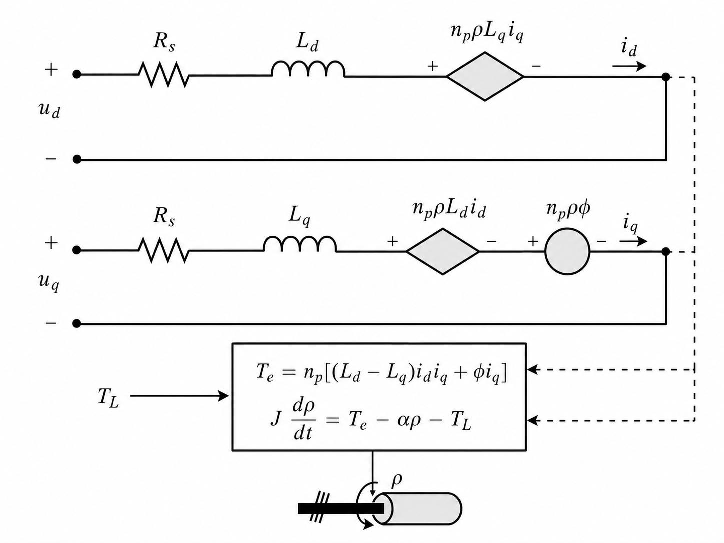
\includegraphics[width=0.62\textwidth]{figs/pmsm_model.pdf}
	\caption{Schematic diagram of the PMSM model.}
	\label{fig:pmsm_schematic}
\end{figure}

Based on the IT-2 T-S fuzzy modeling approach and the state vector $x(t) = [i_d(t), i_q(t), \rho(t)]^{\mathrm{T}}$, where $i_d(t)$ and $i_q(t)$ denote the direct- and quadrature-axis currents and $\rho(t)$ denotes the motor angular velocity, the system is represented as
\begin{equation} 
	\label{eq:example_euqation}
	\left\{
	\begin{aligned}
		\dot{x}(t) &= \sum_{m=1}^{r} \sum_{n=1}^{r} h_m(x_3(t)) h_n(x_3(t)) \Big\{ A_{m} x(t) + B_{m} F_i K_{n} \big[ (1-\theta(t_k h)) x(t_k h) + \theta(t_k h) f(x(t_k h)) \big] + E_{m} w(t) \Big\} \\
		z(t) &= \sum_{m=1}^{r} \sum_{n=1}^{r} h_m(x_3(t)) h_n(x_3(t)) C x(t) 
	\end{aligned}
	\right.
\end{equation}
where the premise variable is chosen as $x_3(t)=\rho(t)$. The corresponding system matrices are
\begin{align}
	\label{eq:system_matrices}
	A_1 &= \begin{bmatrix} -1 & c_1 + d_1 & 0 \\ -(c_1 + d_1) & -1 & \chi \\ 0 & \phi & -\phi \end{bmatrix}, \quad
	A_2 = \begin{bmatrix} -1 & c_1 - d_1 & 0 \\ -(c_1 - d_1) & -1 & \chi\\ 0 & \phi & -\phi \end{bmatrix} \\
	B_1  &= B_2=\begin{bmatrix}1&1&0\end{bmatrix}^{\mathrm T},\quad
	E_1=E_2=\begin{bmatrix}0&0&-1\end{bmatrix}^{\mathrm T},\quad
	C=\begin{bmatrix}1&0&0\end{bmatrix}.
\end{align}
with $c_1$, $d_1$, $\chi$, and $\phi$ being PMSM-related parameters.

The lower and upper FMFs are selected as $\underline{h}_1(x_3(t)) = 0.5 \left( 1 - \frac{5 - x_3(t)}{d_1} \right)$, $\overline{h}_1(x_3(t)) = 0.5 \left( 1 - \frac{0 - x_3(t)}{d_1} \right)$, $\underline{h}_2(x_3(t)) = 1 - \overline{h}_1(x_3(t))$, and $\overline{h}_2(x_3(t)) = 1 - \underline{h}_1(x_3(t))$. The weighting coefficient functions are chosen as $\underline{l}_1(x_3(t))=\overline{l}_2(x_3(t))=\cos^{2}(x_3(t))$ and $\overline{l}_1(x_3(t))=\underline{l}_2(x_3(t))=\sin^{2}(x_3(t))$.

Additionally, the transition rate matrix of the Markov process describing actuator failures is chosen as $\Pi = [\lambda_{ij}]_{2 \times 2} = \begin{bmatrix} -0.6 & 0.6 \\ 1.2 & -1.2 \end{bmatrix}$. The actuator-failure parameters are set to $F_{10} = 0.9$, $F_{11} = 0.1$ for mode 1, and $F_{20} = 0.8$, $F_{21} = 0.2$ for mode 2. In addition, the external disturbance is specified by
$w(t)=0.5\sin(t)$, while the deception attack signal is defined as
$f(x(t))=[0.2\tanh(x_1(t)),\,0.3\tanh(x_2(t)),\,0.25\tanh(x_3(t))]^{\mathrm{T}}$,
which satisfies Assumption~\ref{assump:attack_bound} with $\bar{L}=0.3$.

\begin{figure}[H]
	\centering
	\begin{minipage}{0.45\linewidth}
		\centering 
		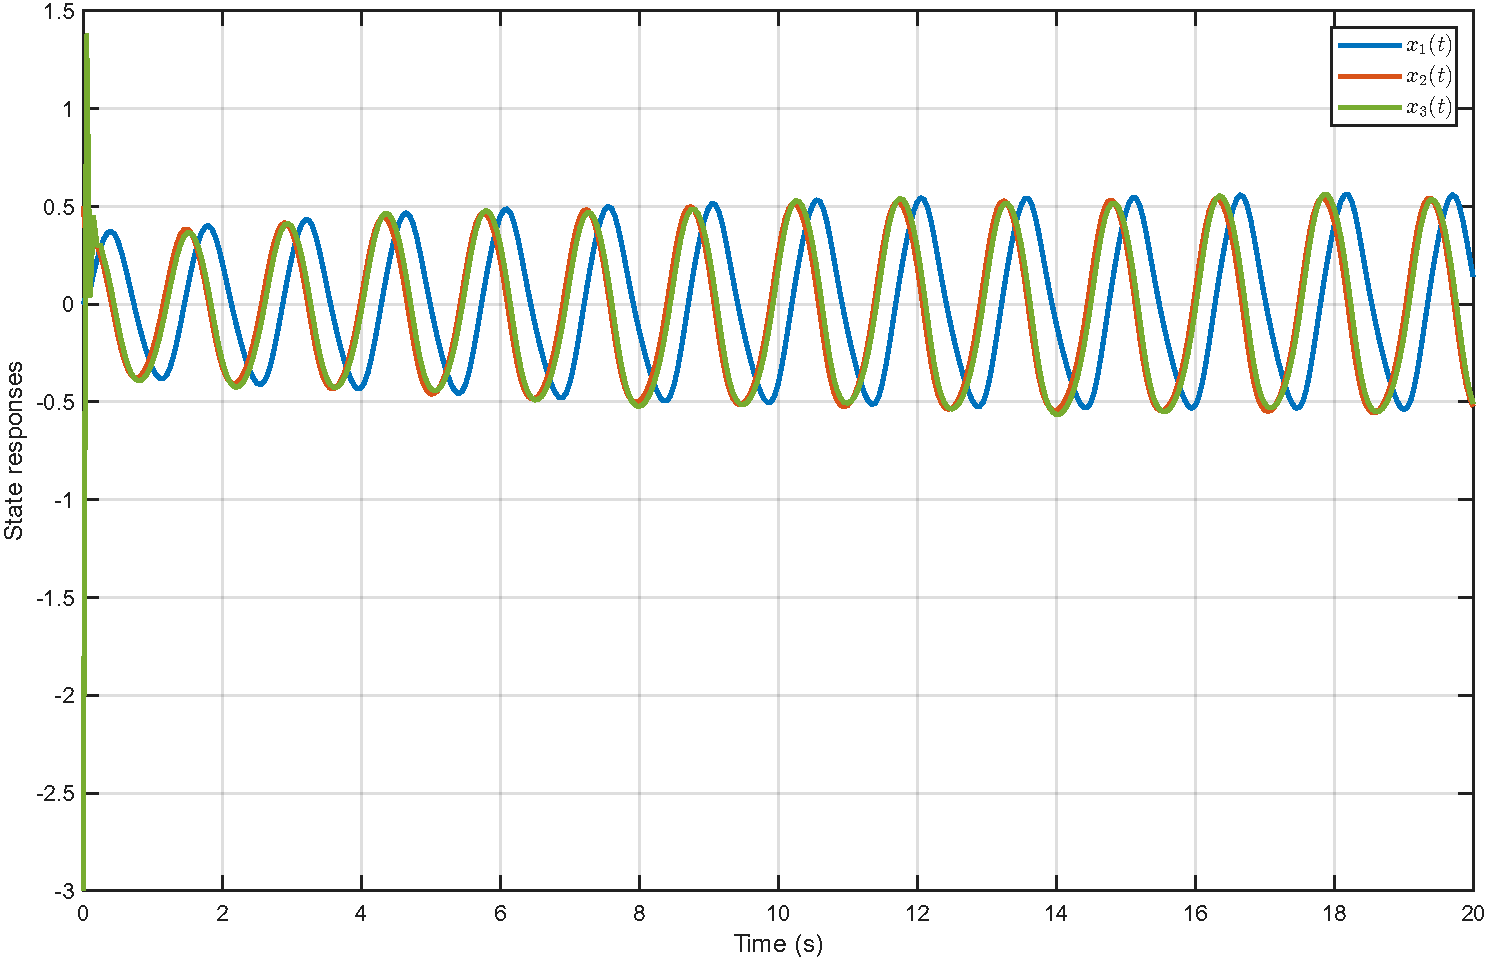
\includegraphics[width=0.9\textwidth]{figs/x(t)_not_u(t).pdf}
		\caption{State responses $x(t)$ without control input.}
		\label{fig2}
	\end{minipage}
	\begin{minipage}{0.45\linewidth}
		\centering 
		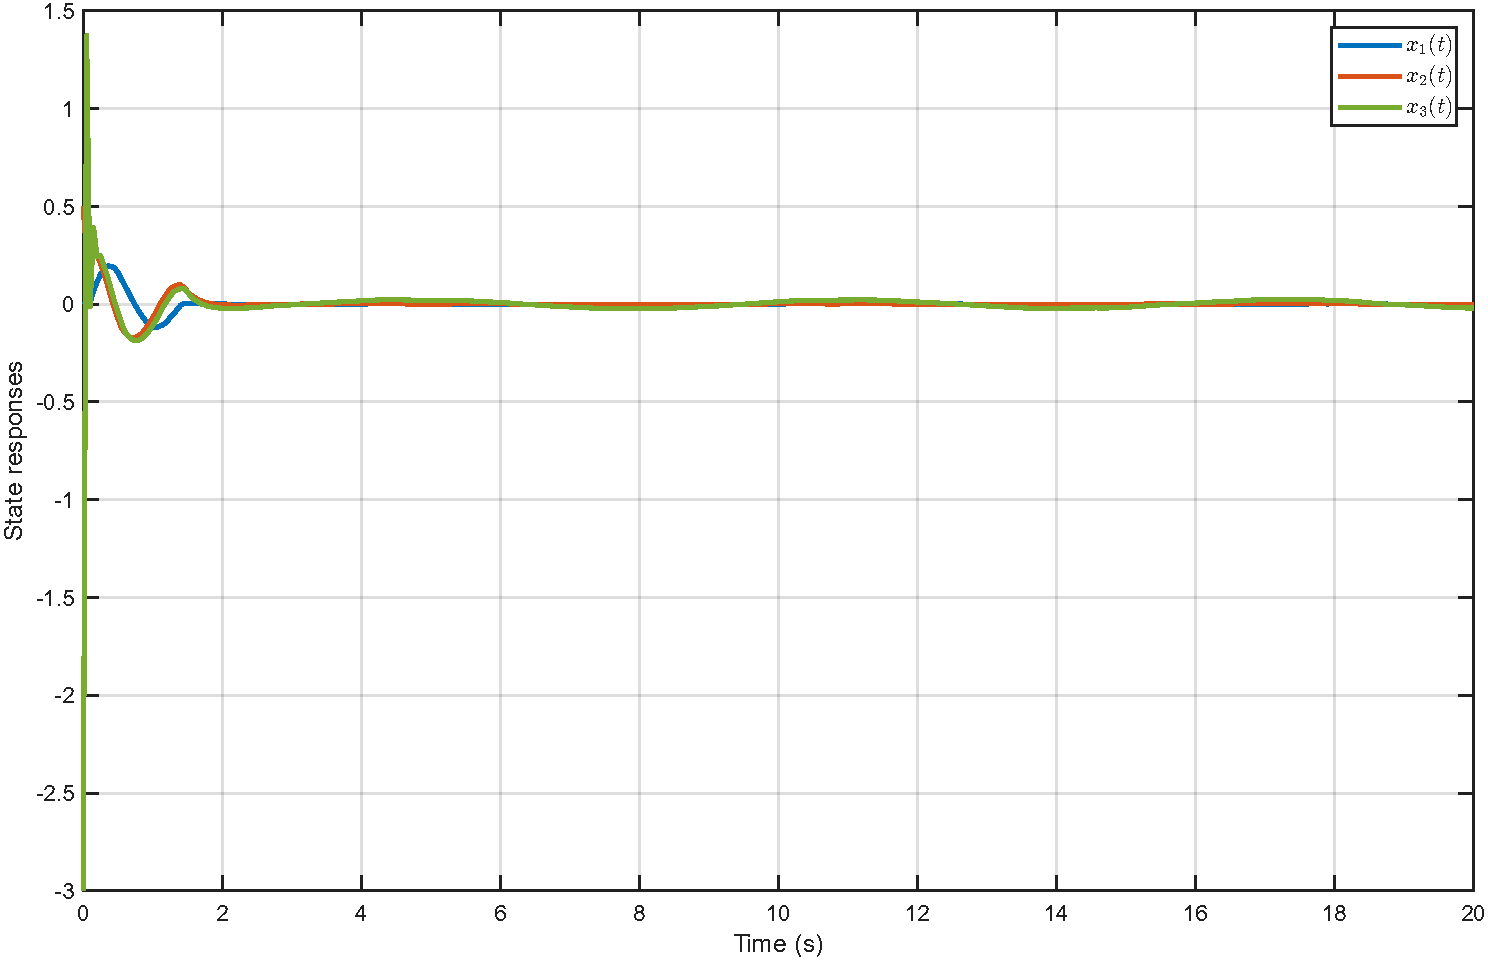
\includegraphics[width=0.9\textwidth]{figs/x(t).pdf}
		\caption{State responses $x(t)$ with control input.}
		\label{fig3}
	\end{minipage}
\end{figure}

With the scalar parameters chosen as $\tau = 0.8$, $\xi_1 = 0.01$, $\xi_2 = 0.01$, $h = 0.05$, $\gamma=2$, $\sigma = 4$, 
$\bar{\theta} = 0.4$, $\phi = 25$, $\chi= 1.1$, $d_1 = 12$, and $c_1 = 5$, 
the LMIs in Theorem \ref{thm3} are solved under the constraint set
$
		\mathcal{C}_1 = \big\{
		\widetilde{P}_{iv}-\widetilde{P}_{ir} \geq 0,\ 
		\widetilde{M}_{v}-\widetilde{M}_{r} \geq 0,\ 
		\widetilde{R}_{1v}-\widetilde{R}_{1r} \geq 0,
		\widetilde{R}_{2v}-\widetilde{R}_{2r} \leq 0,\ 
		\widetilde{H}_{1v}-\widetilde{H}_{1r} \geq 0,\ 
		\widetilde{H}_{2v}-\widetilde{H}_{2r} \geq 0
		\big\},
$
which gives the controller gains and weighting matrix as follows:
\begin{equation*}
	\begin{aligned}
		K_{11} =
		\begin{bmatrix}
			-3.1181 & -3.9483 & -0.0182
		\end{bmatrix}, 
		K_{12} =
		\begin{bmatrix}
			-3.4620 & -4.5144 & -0.0619
		\end{bmatrix}, 
		S_1 =
		\begin{bmatrix}
			9.7356 & 10.9579 & -0.0543 \\
			10.9579 & 14.8266 & -0.7842 \\
			-0.0543 & -0.7842 & 0.8651
		\end{bmatrix}.
	\end{aligned}
\end{equation*}

Under the same system matrices and scalar parameters, the LMIs are further solved with the constraint set
$
		\mathcal{C}_2 = \big\{
		\widetilde{P}_{iv}-\widetilde{P}_{ir} \leq 0,\ 
		\widetilde{M}_{v}-\widetilde{M}_{r} \leq 0,\ 
		\widetilde{R}_{1v}-\widetilde{R}_{1r} \leq 0,
		\widetilde{R}_{2v}-\widetilde{R}_{2r} \geq 0,\ 
		\widetilde{H}_{1v}-\widetilde{H}_{1r} \leq 0,\ 
		\widetilde{H}_{2v}-\widetilde{H}_{2r} \leq 0
		\big\},
$
yielding the following controller gains and weighting matrix:
\begin{equation*}
	\begin{aligned}
		K_{21} =
		\begin{bmatrix}
			-3.3108 & -3.8233 & -0.2673
		\end{bmatrix}, 
		K_{22} =
		\begin{bmatrix}
			-3.4639 & -4.0632 & -0.3020
		\end{bmatrix}, 
		S_2 =
		\begin{bmatrix}
			9.4184 & 10.1425 & 0.6210 \\
			10.1425 & 12.5051 & -0.0274 \\
			0.6210 & -0.0274 & 0.8892
		\end{bmatrix}.
	\end{aligned}
\end{equation*}

\begin{figure}[H]
	\centering
	\begin{minipage}{0.45\linewidth}
		\centering 
		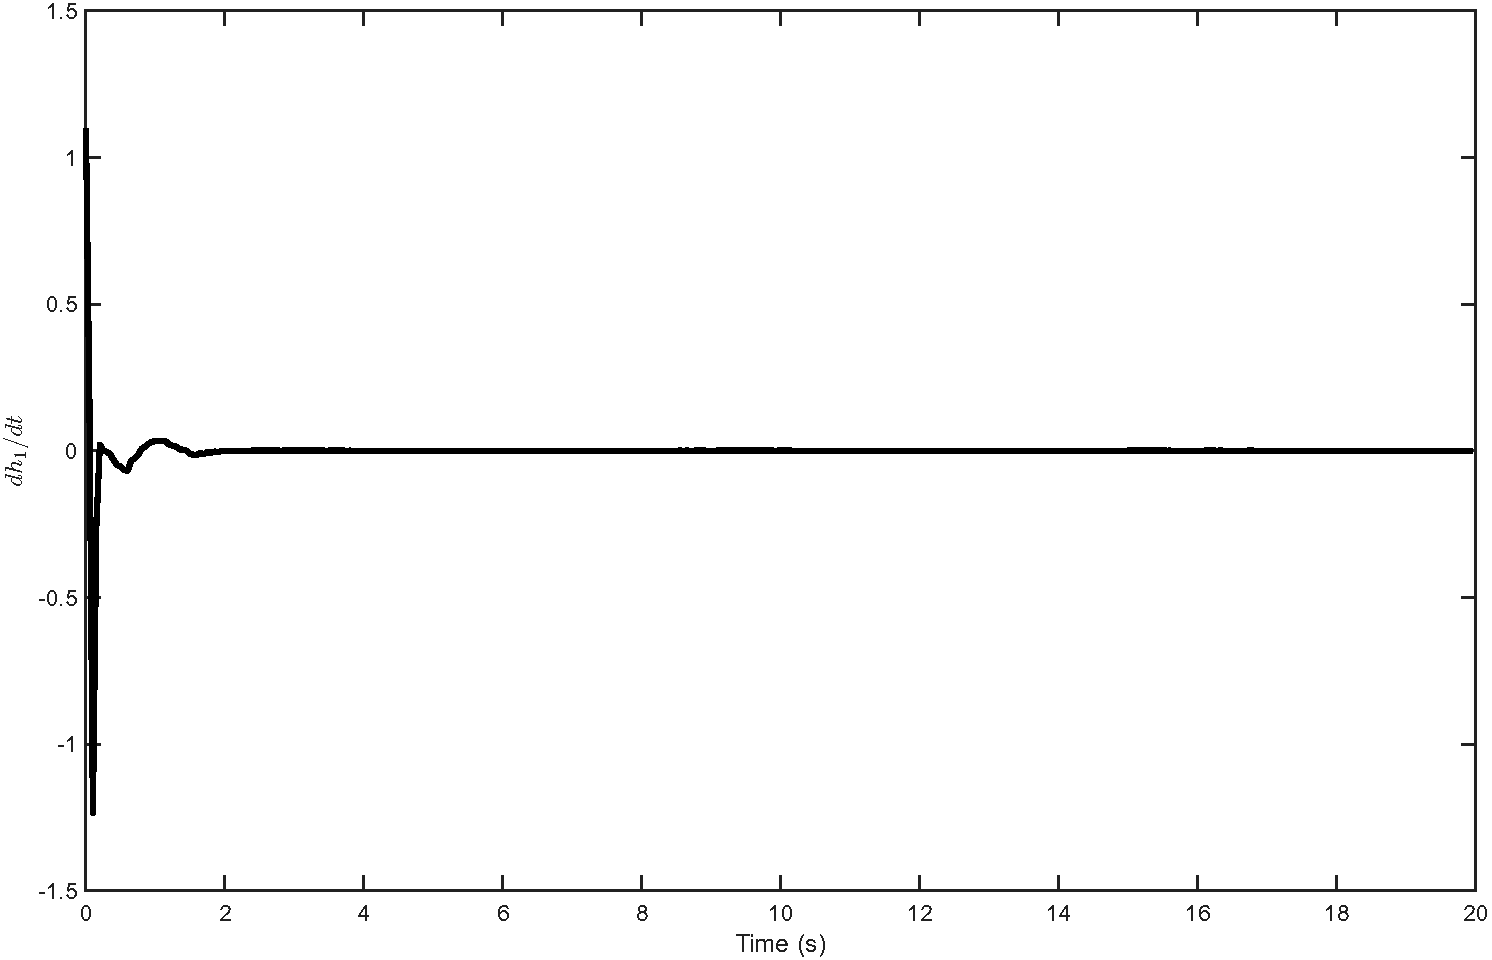
\includegraphics[width=0.9\textwidth]{figs/h_1_dot.pdf}
		\caption{Evolution of $\dot{h}_1(t)$.}
		\label{fig4}
	\end{minipage}
	\begin{minipage}{0.45\linewidth}
		\centering 
		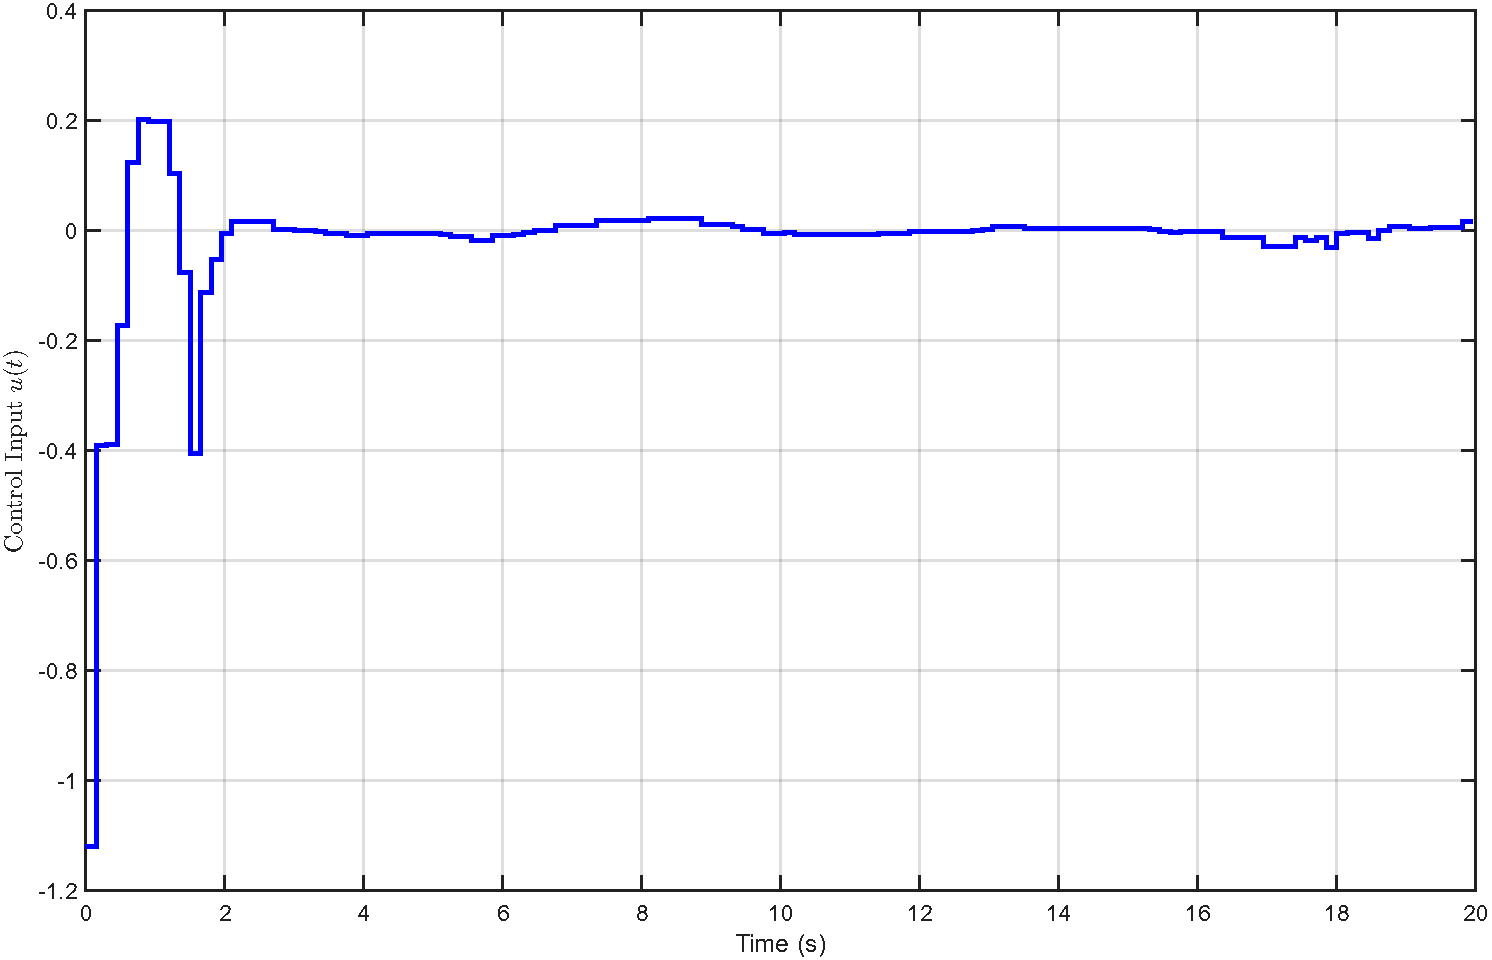
\includegraphics[width=0.9\textwidth]{figs/u(t).pdf}
		\caption{Control input $u(t)$.}
		\label{fig5}
	\end{minipage}
\end{figure}

\begin{figure}[H]
	\centering
	\begin{minipage}{0.45\linewidth}
	\centering 
	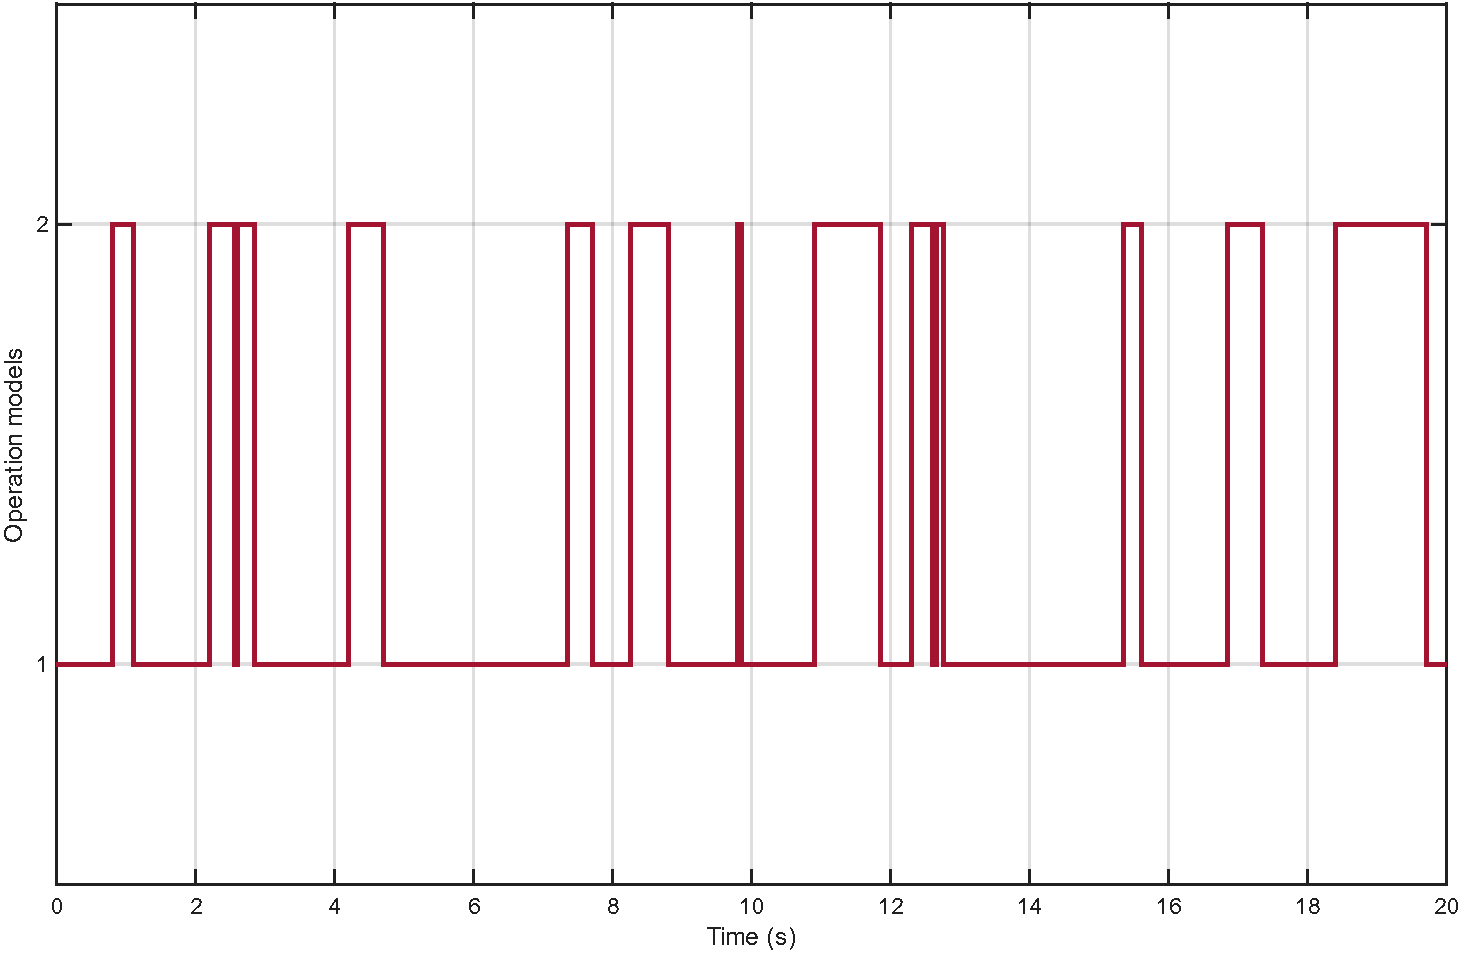
\includegraphics[width=0.9\textwidth]{figs/actuator_fault.pdf}
	\caption{Evolution of the actuator fault mode $r(t)$.}
		\label{fig6}
	\end{minipage}
	\begin{minipage}{0.45\linewidth}
	\centering 
	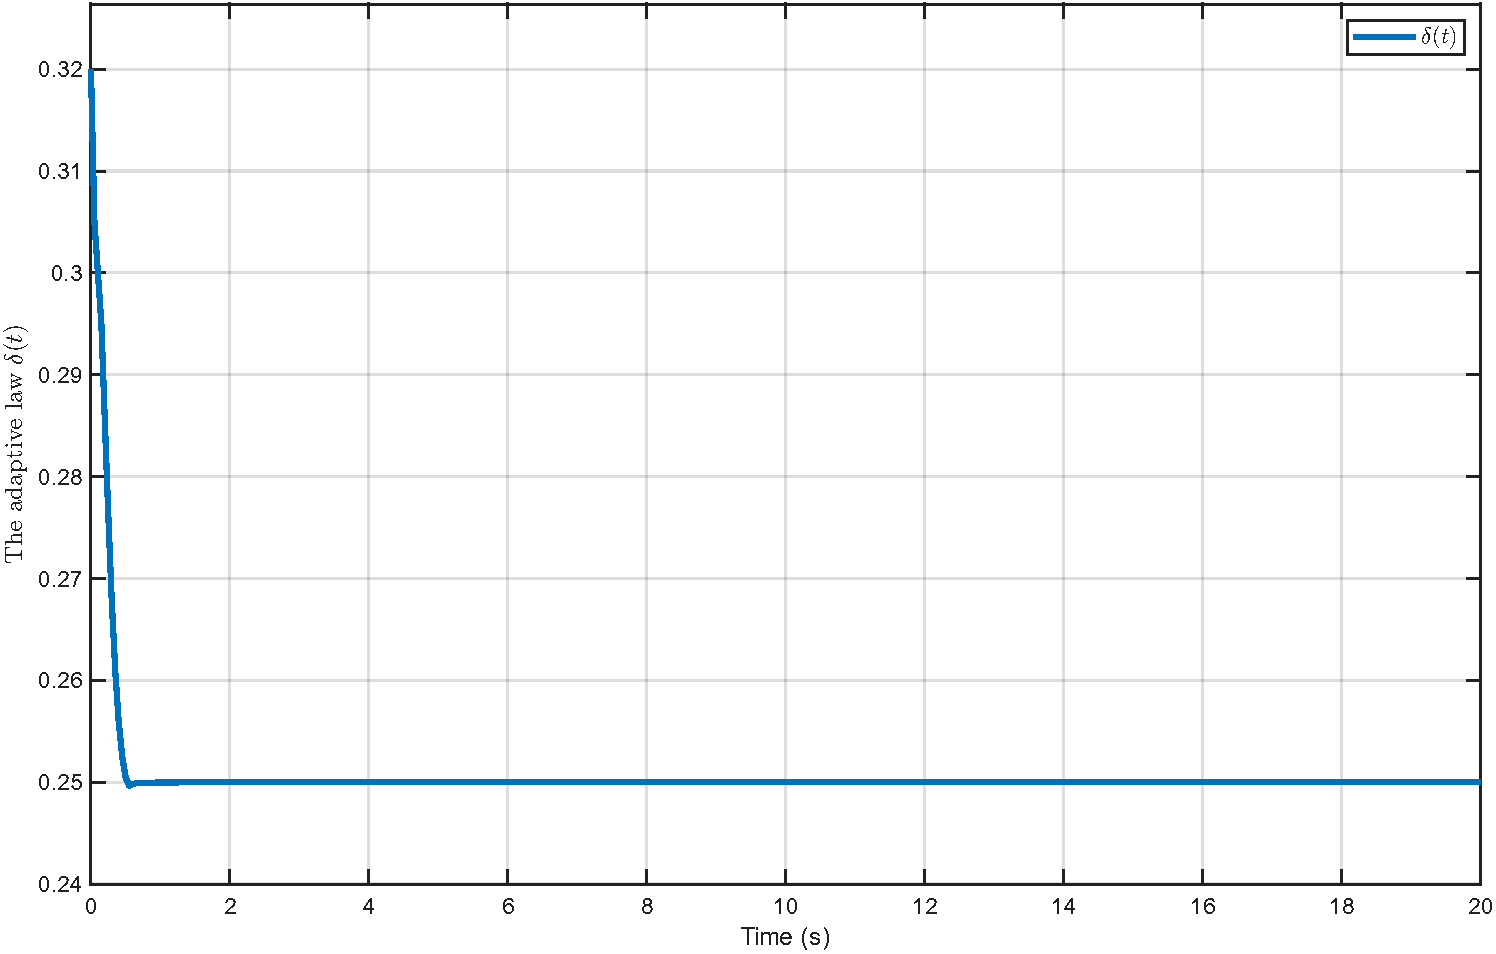
\includegraphics[width=0.9\textwidth]{figs/AETM_law.pdf}
	\caption{Adaptive threshold $\delta(t)$.}
	\label{fig7}
	\end{minipage}
\end{figure}

\begin{figure}[htbp]
	\centering
	\begin{minipage}{0.48\linewidth}
		\centering 
		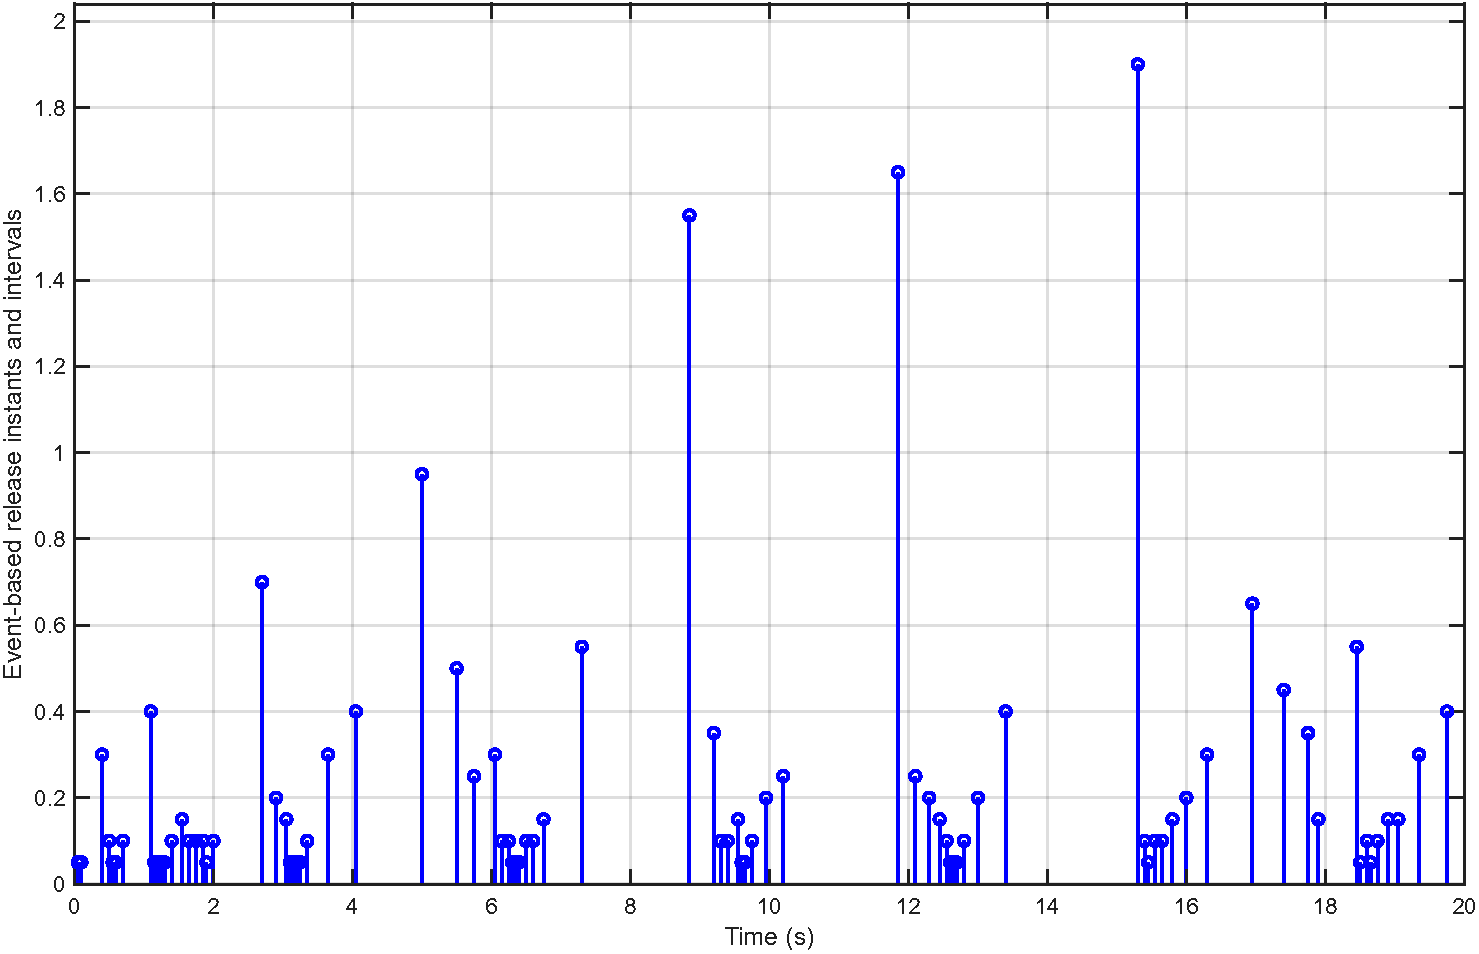
\includegraphics[width=0.9\textwidth]{figs/event_tri_time.pdf}
		\caption{Release instants and release intervals.}
		\label{fig8}
	\end{minipage}
\end{figure}

With the initial state $x(0)=\begin{bmatrix}0 & 0.5 & -3\end{bmatrix}^{\mathrm{T}}$, 
Figs.~\ref{fig2} and~\ref{fig3} present the open-loop and closed-loop state responses, respectively. 
It can be observed that the open-loop system exhibits evident oscillatory behavior, whereas the proposed controller drives all system states to equilibrium despite deception attacks and stochastic actuator failures.

Figs.~\ref{fig4}--\ref{fig8} provide further simulation results.
Fig.~\ref{fig4} depicts the time evolution of $\dot{h}_1(t)$. Its bounded transient behavior and convergence to zero indicate that the membership-function derivative information can be effectively exploited in the region-dependent piecewise control design.
Fig.~\ref{fig5} presents the control signal $u(t)$ generated by the proposed controller, which remains bounded throughout the simulation.
Fig.~\ref{fig6} illustrates the stochastic switching of the actuator-failure mode $r(t)$, reflecting the random variation of actuator operating conditions.
Fig.~\ref{fig7} shows the evolution of the adaptive threshold $\delta(t)$, which gradually approaches the equilibrium value $1/\sigma=0.25$.
The corresponding release instants and inter-event intervals are shown in Fig.~\ref{fig8}.
 
To further demonstrate how effectively the proposed AETM reduces communication,
Table~\ref{tab:sigma_effect} compares the transmitted packet counts for the proposed AETM and the time-triggered mechanism under different values of $\sigma$.
Under the time-triggered mechanism, all 400 sampled data packets are transmitted, whereas under the proposed AETM, only the data packets satisfying the triggering condition are released.
These results confirm that the proposed AETM significantly reduces the number of data transmissions.
\begin{table}[htbp]
	\centering
	\caption{Comparison of communication burden under different values of $\sigma$}
	\label{tab:sigma_effect}
	\begin{tabular}{cccc}
		\toprule
		$\sigma$ & Time-triggered mechanism & Proposed AETM & Saving rate \\
		\midrule
		4  & 400 & 85  & 78.75\% \\
		6  & 400 & 113 & 71.75\% \\
		10 & 400 & 136 & 66.00\% \\
		20 & 400 & 164 & 59.00\% \\
		\bottomrule
	\end{tabular}
\end{table}

\iffalse
\begin{table}[htbp]
	\centering
	\caption{Comparison of communication burden under different values of $\sigma$}
	\label{tab:sigma_effect}
	% m{宽度} 可以让文字在格子内水平+垂直居中，<{\centering} 确保强制居中
	\begin{tabular}{ c | >{\centering\arraybackslash}m{3.8cm} | >{\centering\arraybackslash}m{2.8cm} | c }
		\hline % 用普通的 hline，确保竖线上下完全接上，不留空隙
		$\sigma$ & Time-triggered mechanism & Proposed AETM & Saving rate \\
		\hline
		2  & 600 & 74  & 87.67\% \\
		5  & 600 & 100 & 83.33\% \\
		10 & 600 & 122 & 79.67\% \\
		15 & 600 & 123 & 79.50\% \\
		\hline
	\end{tabular}
\end{table}
\fi

Therefore, the results of Example~\ref{exm1} confirm that the co-design method achieves closed-loop stability while effectively reducing the communication burden.

\end{example}

\begin{example}\label{exm2}
To further assess the developed method, the following IT-2 fuzzy CPS is considered, with its system parameters specified as follows:
\begin{align*}
	A_1 &= \begin{bmatrix}
		-1.1 & 0.2 & 1.3 \\
		0.2 & -1.5 & 0.1 \\
		0.8 & 0.1 & -0.4
	\end{bmatrix}, \quad
	A_2 = \begin{bmatrix}
		-1.8 & 0.4 & 0.1 \\
		0.3 & -2.0 & 0.1 \\
		0.5 & 0.2 & -0.3
	\end{bmatrix}, \quad
	B_1 = B_2 = \begin{bmatrix} 1.0 & 0.5 & 0.5 \end{bmatrix}^{\mathrm{T}}, \\
	E_1 &= E_2 =
	\begin{bmatrix}
		0.1 & 0 & 0 \\
		0 & 0 & 0.1 \\
		0 & 0.1 & 0.2
	\end{bmatrix}, \quad
	C = \begin{bmatrix} 0.1 & 0 & 0 \end{bmatrix}.
\end{align*}

The lower and upper FMFs are given by $\underline{h}_1(x_1(t)) = 1 - e^{-\frac{x_1^2(t)}{5}}$, $\overline{h}_1(x_1(t)) = 1 - e^{-\frac{x_1^2(t)}{2}}$, $\underline{h}_2(x_1(t)) = 1 - \overline{h}_1(x_1(t))$, and $\overline{h}_2(x_1(t)) = 1 - \underline{h}_1(x_1(t))$. The weighting coefficient functions are selected as $\underline{l}_1(x_1(t))=\overline{l}_2(x_1(t))=\cos^{2}(x_1(t))$ and $\overline{l}_1(x_1(t))=\underline{l}_2(x_1(t))=\sin^{2}(x_1(t))$. 

The same actuator-failure transition rate matrix, and deception attack signal as in Example~\ref{exm1} are adopted here, whereas the external disturbance input is modified to $w(t) = 0.2[\sin(x_1(t)),\sin(x_2(t)),\sin(x_3(t))]^{\mathrm{T}}$. Unlike Example~\ref{exm1}, where different values of $\sigma$ are compared to examine the effect of the adaptive threshold parameter, Example~\ref{exm2} adopts a fixed parameter setting to further evaluate the proposed method in terms of performance and applicability under a different IT-2 fuzzy system configuration.

\begin{figure}[H]
	\centering
	\begin{minipage}{0.45\linewidth}
		\centering 
		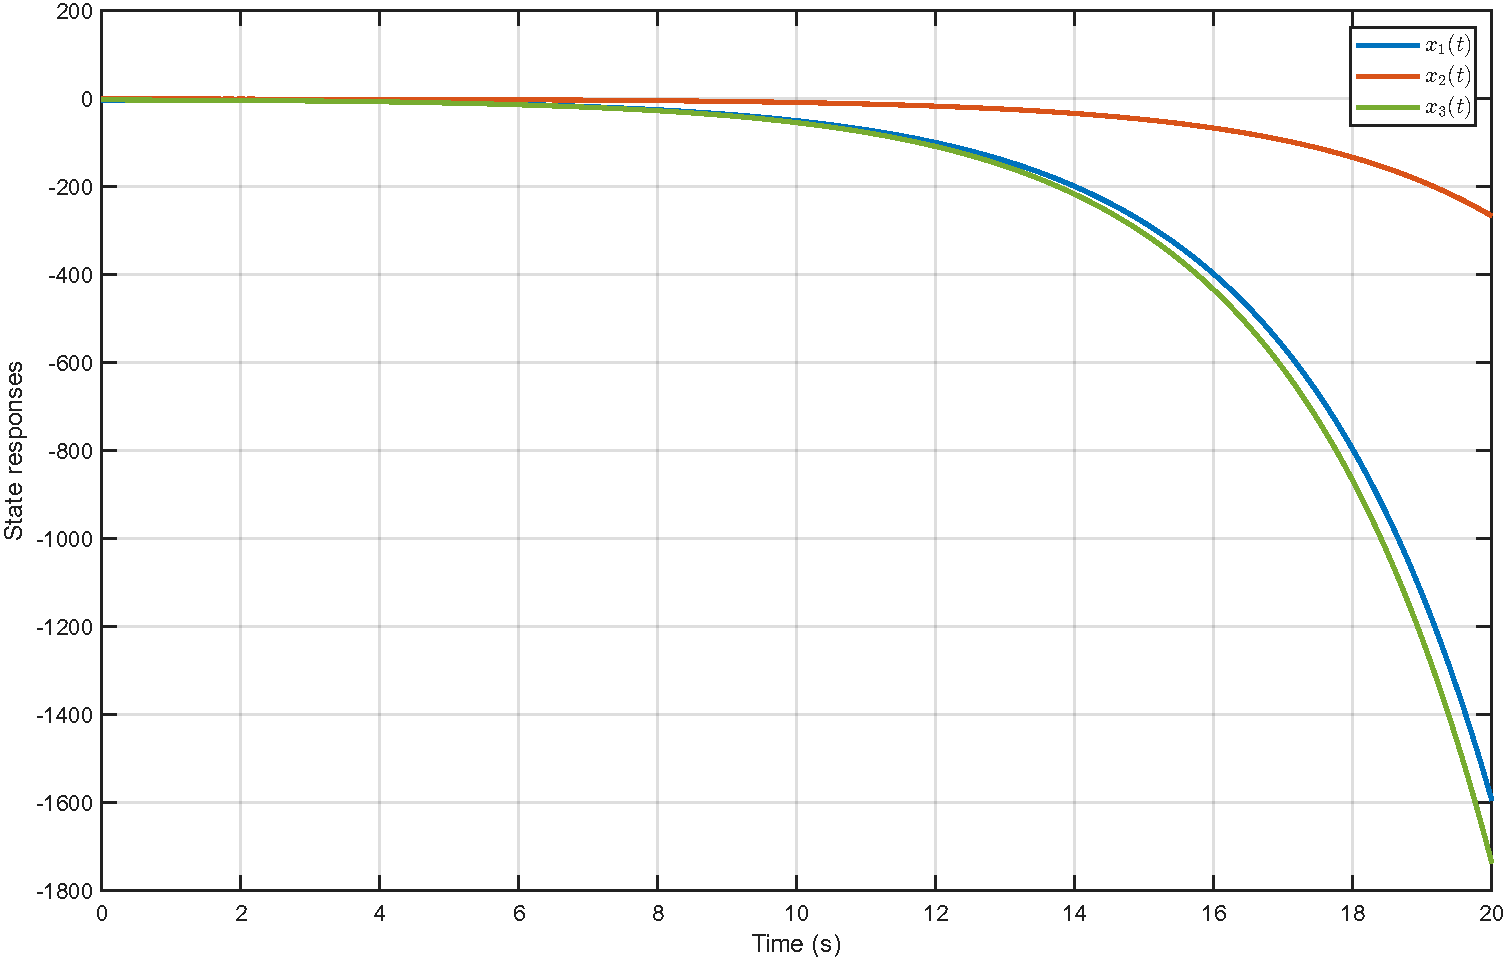
\includegraphics[width=0.9\textwidth]{figs/2_x(t)_not_u(t).pdf}
		\caption{State responses $x(t)$ without control input.}
		\label{fig10}
	\end{minipage}
	\begin{minipage}{0.45\linewidth}
		\centering 
		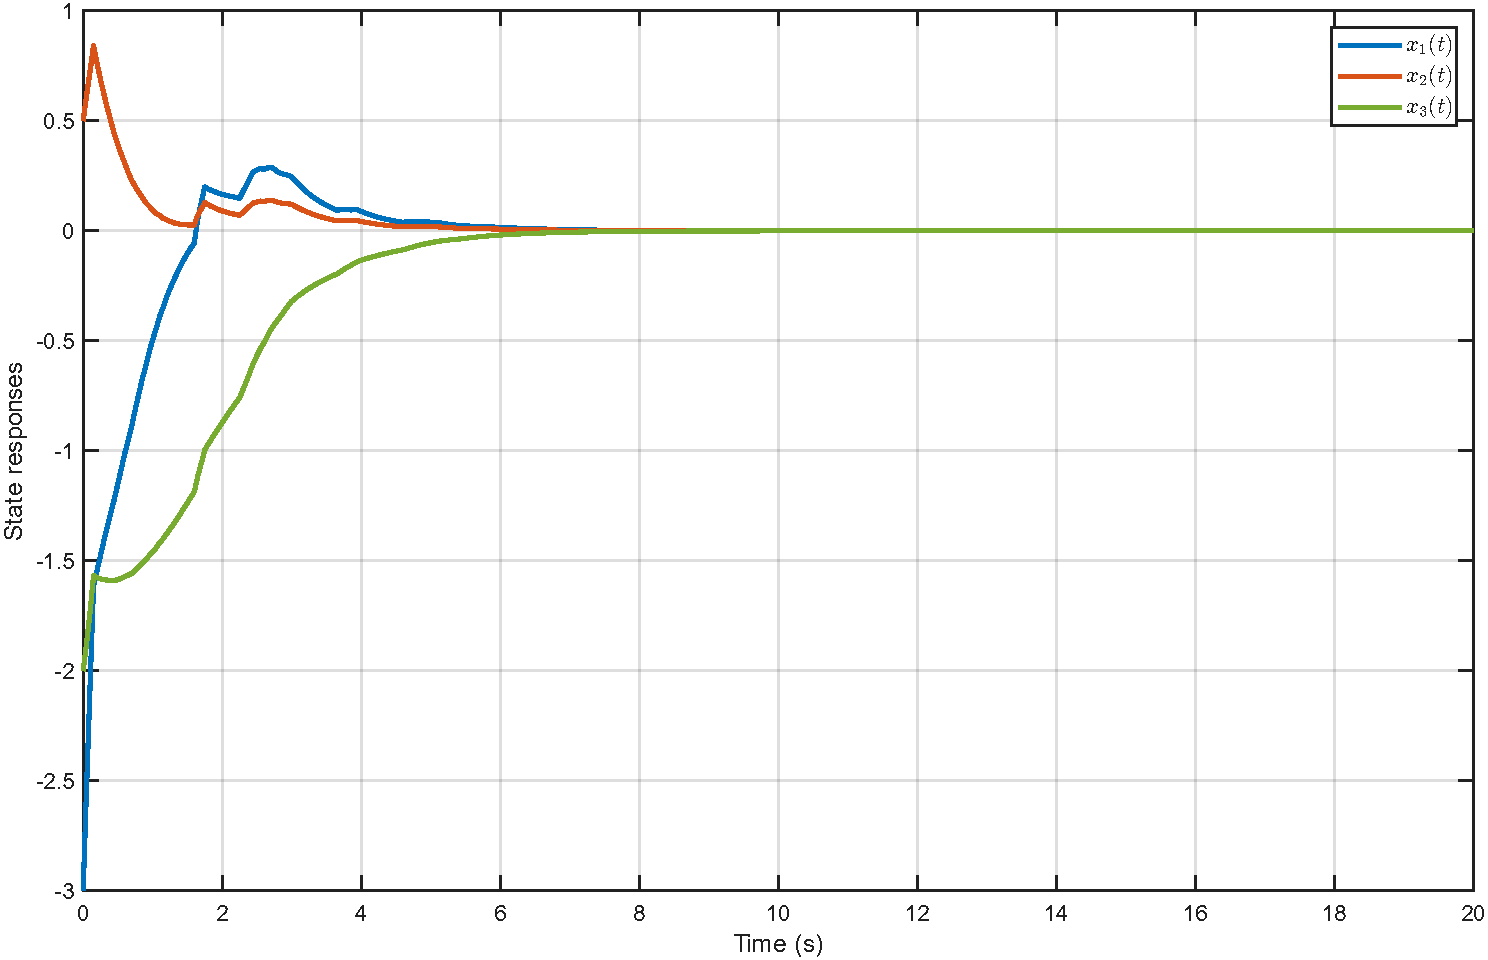
\includegraphics[width=0.9\textwidth]{figs/2_x(t).pdf}
		\caption{State responses $x(t)$ with control input.}
		\label{fig11}
	\end{minipage}
\end{figure}

Using the design parameters $\tau = 2$, $\xi_1 = 2$, $\xi_2 = 4$, $h = 0.05$, $\sigma = 10$, $\gamma = 2$, with $\bar{\theta} = 0.4$, the LMIs of Theorem~\ref{thm3} are solved subject to the regional constraint
$
\mathcal{C}_1=\{\widetilde{P}_{iv}-\widetilde{P}_{ir} \ge 0, \widetilde{M}_{v}-\widetilde{M}_{r} \ge 0, 
\widetilde{R}_{1v}-\widetilde{R}_{1r} \ge 0,
\widetilde{R}_{2v}-\widetilde{R}_{2r} \leq 0,
\widetilde{H}_{1v}-\widetilde{H}_{1r} \ge 0, 
\widetilde{H}_{2v}-\widetilde{H}_{2r} \ge 0\},
$
which gives
\begin{equation*}       
	\begin{aligned}     
		K_{11} &=
		\begin{bmatrix}
			-0.4761 & -0.2864 & -0.1834
		\end{bmatrix}, 
		K_{12} =     
		\begin{bmatrix}
			-0.7349 & -0.4756 & -0.4822
		\end{bmatrix}, 
		S_1 =
		\begin{bmatrix}
		2.6034  & 0.5325 & 0.3168 \\
		0.5325 &  3.4680 & 0.6784 \\
		0.3168 & 0.6784 &  2.5486
		\end{bmatrix}
	\end{aligned}
\end{equation*}

Similarly, for the complementary region
$
\mathcal{C}_2=\{\widetilde{P}_{iv}-\widetilde{P}_{ir} \le 0, \widetilde{M}_{v}-\widetilde{M}_{r} \le 0, 
\widetilde{R}_{1v}-\widetilde{R}_{1r} \le 0, 
\widetilde{R}_{2v}-\widetilde{R}_{2r} \ge 0, 
\widetilde{H}_{1v}-\widetilde{H}_{1r} \le 0, 
\widetilde{H}_{2v}-\widetilde{H}_{2r} \le 0\},
$
the obtained controller gains are
\begin{equation*}           
	\begin{aligned}
		K_{21} &=
		\begin{bmatrix}
			-1.0727 & -0.7452 & -0.7040
		\end{bmatrix},
		K_{22} =      
		\begin{bmatrix}
			-0.7000  & -0.4550 & -0.4787
		\end{bmatrix}, 
		S_2 =
		\begin{bmatrix}
		3.9273  &  0.5239 & 0.2921 \\
		0.5239 &  5.6784 & 0.8313 \\
		0.2921 & 0.8313 &  4.0387
		\end{bmatrix}
	\end{aligned}
\end{equation*}

\begin{figure}[H]
	\centering
	\begin{minipage}{0.45\linewidth}
		\centering 
		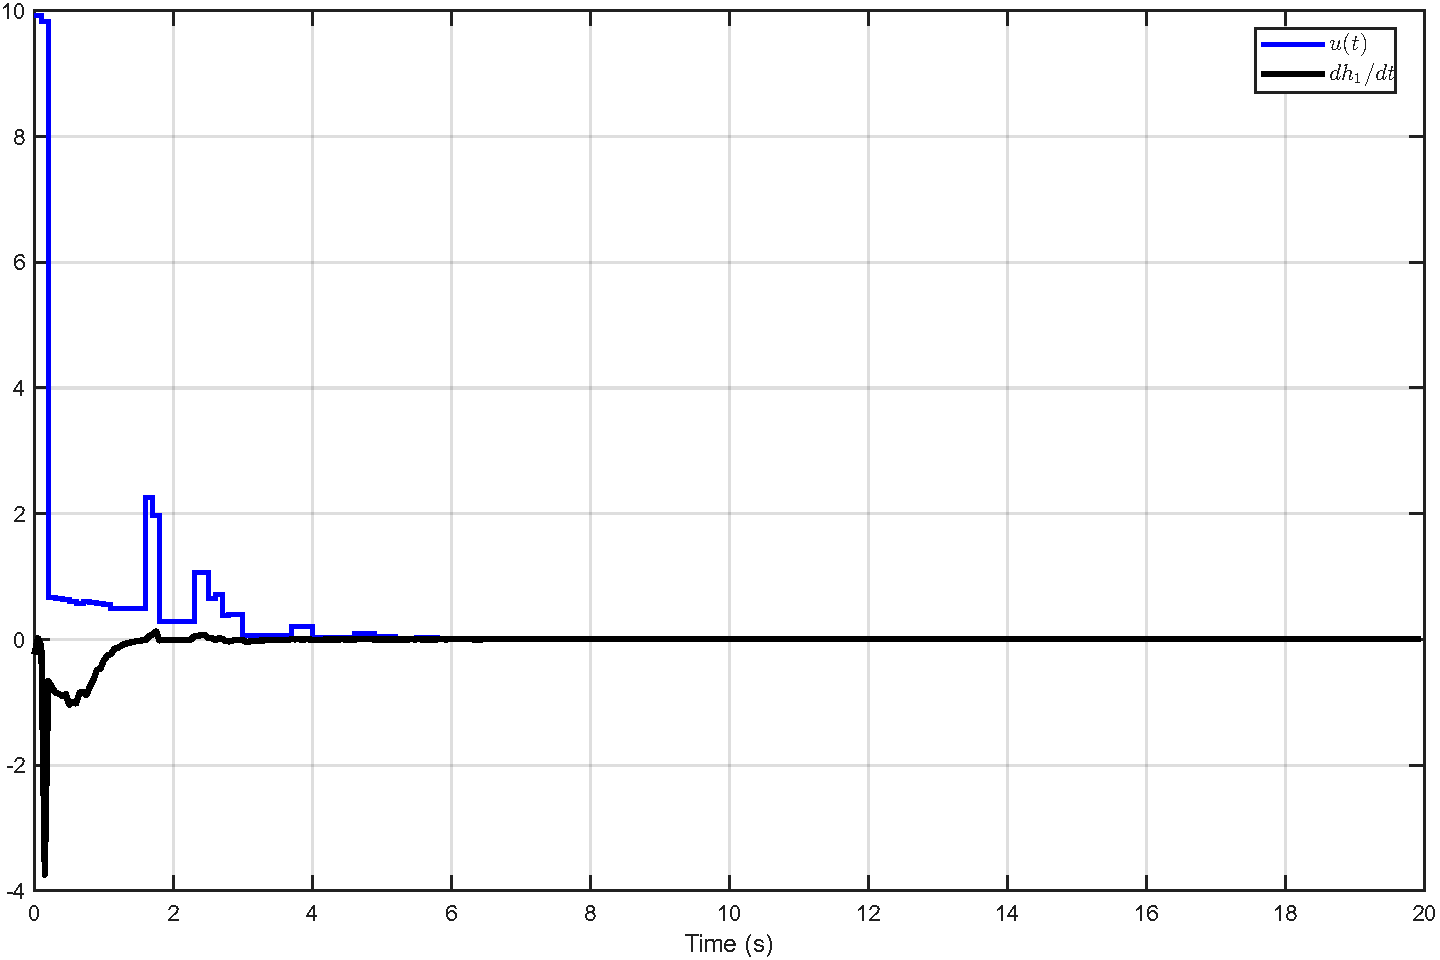
\includegraphics[width=0.9\textwidth]{figs/2_h1_dot_and_ut.pdf}
		\caption{Evolution of $\dot{h}_1(t)$ and control input $u(t)$.}
		\label{fig12}
	\end{minipage}
	\begin{minipage}{0.45\linewidth}
		\centering 
		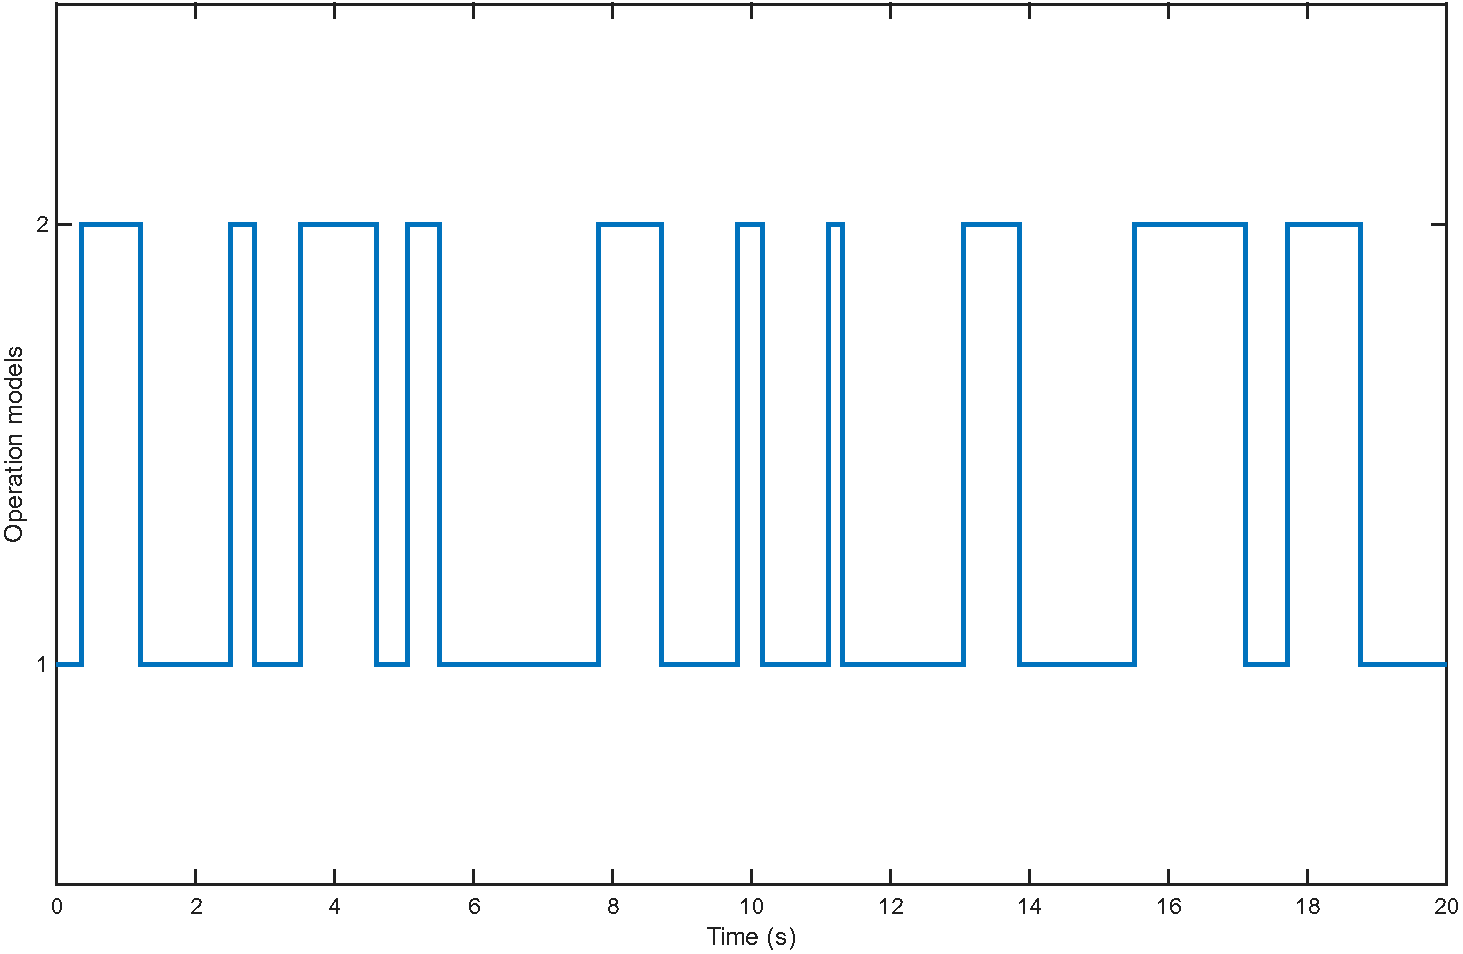
\includegraphics[width=0.9\textwidth]{figs/2_actuator_fault.pdf}
		\caption{Evolution of the actuator fault mode $r(t)$.}
		\label{fig13}
	\end{minipage}
\end{figure}
\begin{figure}[H]
	\centering
	\begin{minipage}{0.45\linewidth}
		\centering 
		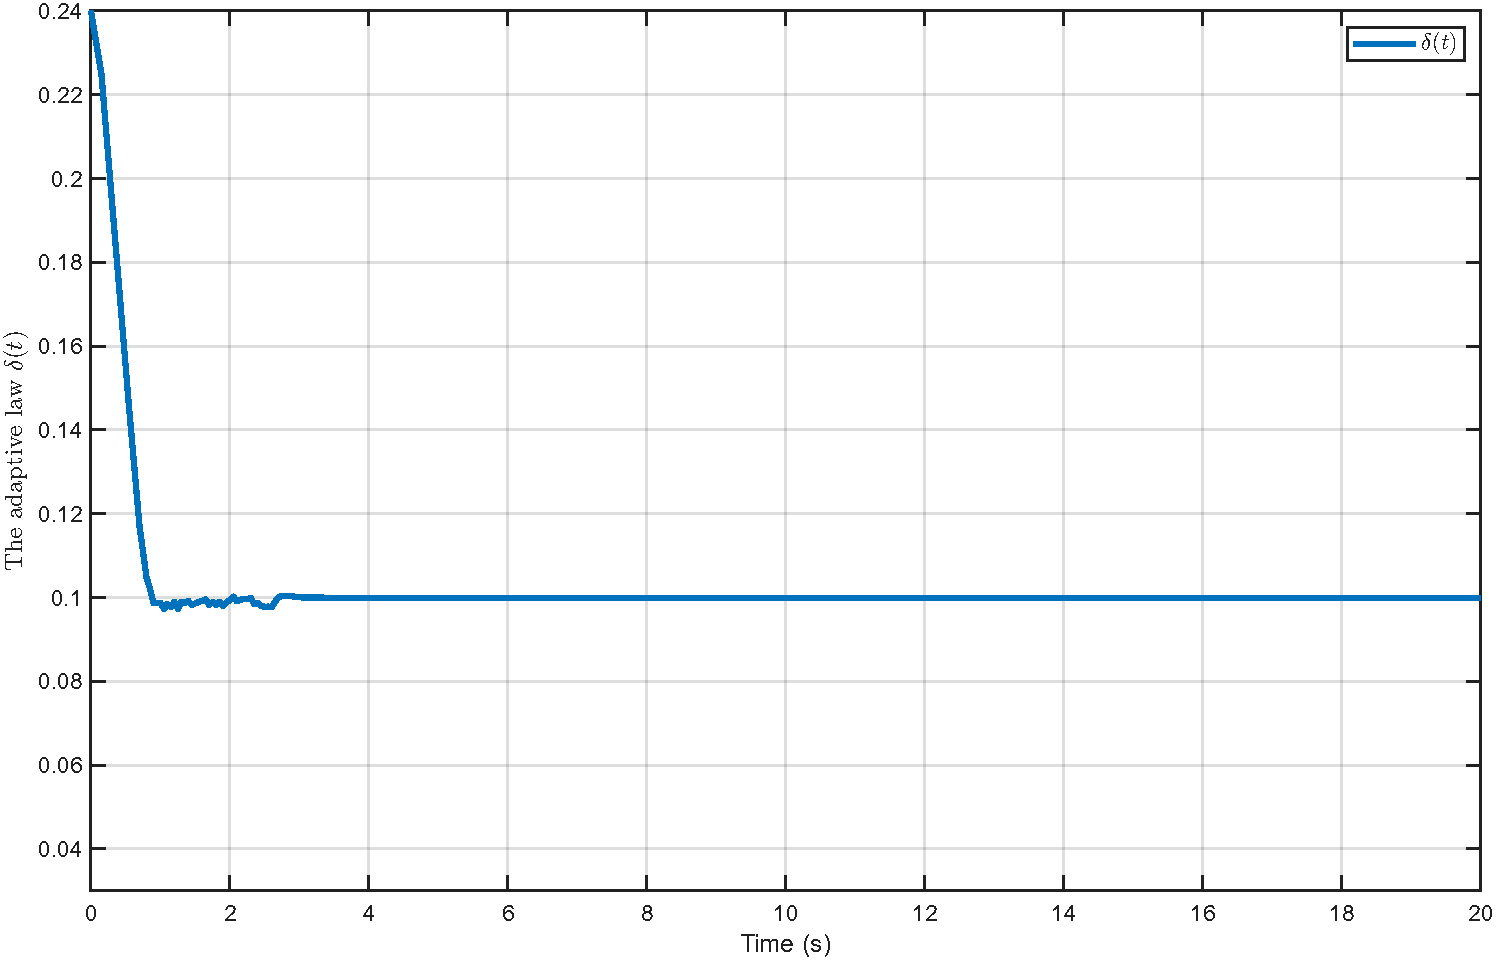
\includegraphics[width=0.9\textwidth]{figs/2_AETM_law.pdf}
		\caption{Adaptive threshold $\delta(t)$.}
		\label{fig14}
	\end{minipage}
	\begin{minipage}{0.45\linewidth}
		\centering 
		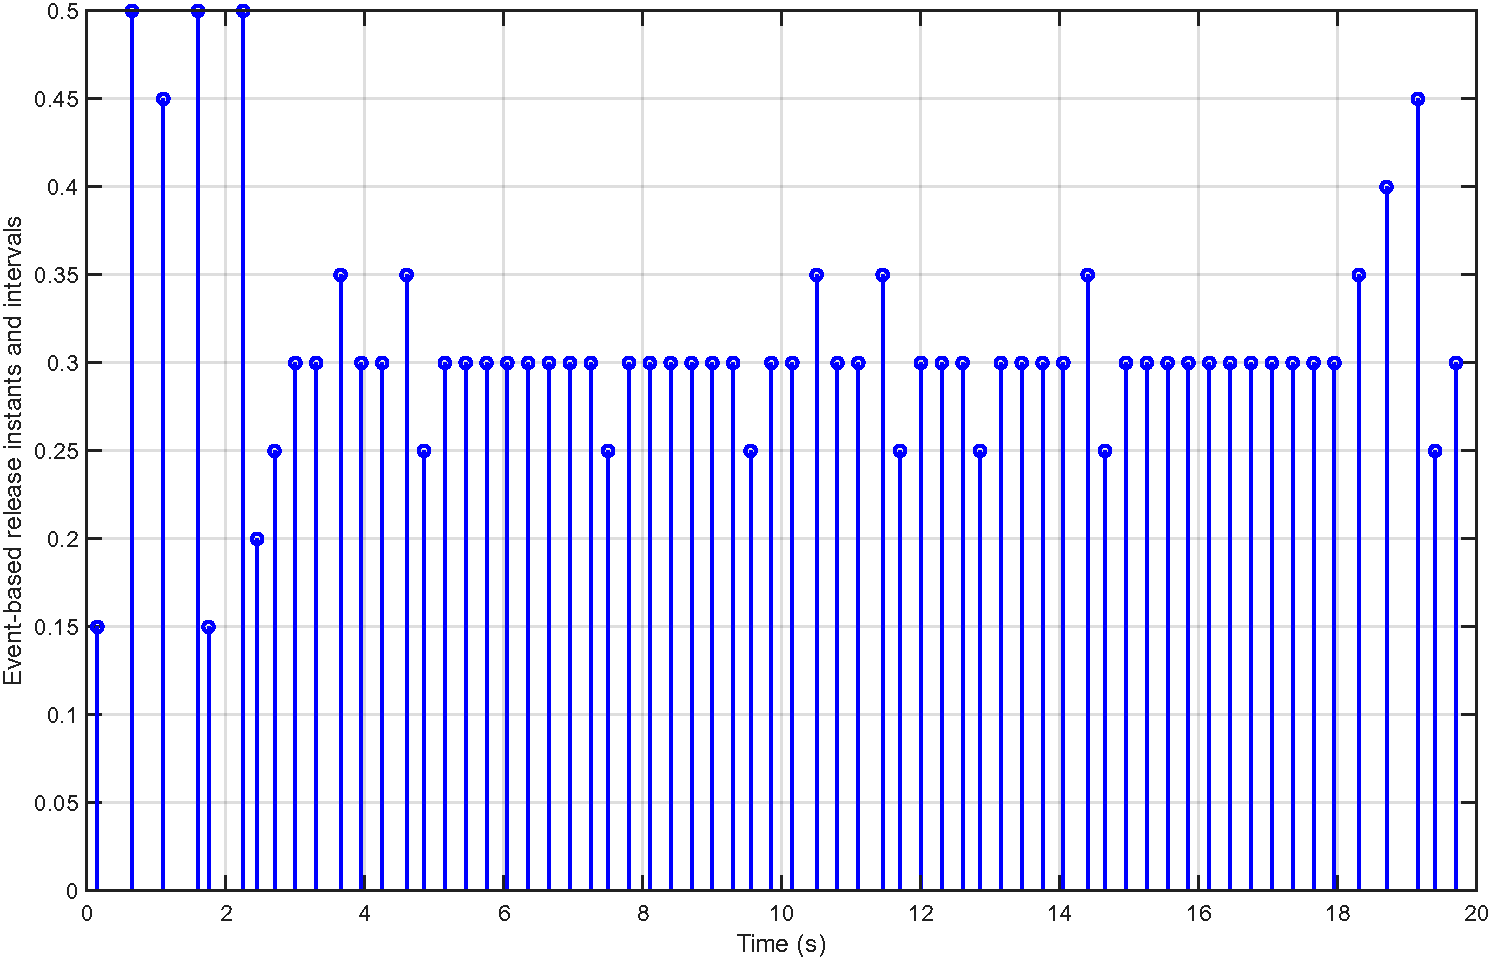
\includegraphics[width=0.9\textwidth]{figs/2_event_tri_time.pdf}
		\caption{Release instants and release intervals.}
		\label{fig15}
	\end{minipage}
\end{figure}

For the same initial state $x(0) = \begin{bmatrix} -3, 0.5, -2 \end{bmatrix}^{\mathrm{T}}$, Figs.~\ref{fig10} and \ref{fig11} compare the responses under open-loop and closed-loop conditions. The open-loop system exhibits a clear divergent behavior, whereas the proposed controller maintains system stability despite deception attacks and Markov-type actuator failures.

Figs.~\ref{fig12} and \ref{fig13} further show the control input, the derivative $\dot{h}_1(t)$, and the stochastic switching of the actuator-failure mode. The control signal remains bounded, and $\dot{h}_1(t)$ approaches zero as the state trajectories converge, which is consistent with the stabilization objective.
Fig.~\ref{fig14} shows that the adaptive threshold $\delta(t)$ again converges to the equilibrium value $1/\sigma = 0.1$, and Fig.~\ref{fig15} records the release instants and inter-event intervals. Under this fixed setting, only 65 transmissions are triggered out of 400 candidate sampling instants, yielding a communication saving rate of $83.79\%$. These results demonstrate that the proposed co-design remains effective for a different IT-2 fuzzy model and offers the same communication-efficiency advantage.

\end{example}

\section{Conclusion} \label{sec5}
This study has addressed adaptive event-triggered $\mathrm{H}_{\infty}$ control of IT-2 fuzzy CPSs affected simultaneously by stochastic deception attacks and Markov-type actuator failures. An AETM has been employed to limit unnecessary data transmissions by updating the triggering threshold online using real-time state-error information. In addition, a region-dependent piecewise fuzzy control strategy has been developed by incorporating derivative information from the membership functions. Based on an FMF-dependent and time-dependent looped functional, stability criteria have been obtained to guarantee closed-loop asymptotic stability while achieving a prescribed $\mathrm{H}_{\infty}$ disturbance attenuation level. The controller gains and adaptive event-triggering weight matrices have been jointly determined through tractable LMIs, while a bounding technique has been employed to address the norm-bounded uncertainty induced by Markov-type actuator failures.

An engineering-motivated PMSM example and a numerical IT-2 fuzzy example have demonstrated the effectiveness and applicability of the developed method. Further research will extend the current IT-2 fuzzy control methodology to observer-based output feedback control, since not all system states are measurable in practical industrial applications. Secure control under more sophisticated cyberattack scenarios, such as DoS attacks, and practical network constraints, such as partially unknown Markov transition probabilities, also deserve further investigation.


\section*{CRediT authorship contribution statement}
{\bf Xiaoqing Li}: Conceptualization, Methodology, Writing--original draft, Writing--review \& editing. %{\bf Kun She}: Experimental platform, Supervision, Software.
{\bf Haoxiang Zhao}: Methodology, Writing--review \& editing. 
{\bf Liang Han}: Conceptualization, Visualization, Writing--review \& editing.
{\bf Jun Cheng}: Conceptualization, Visualization, Writing--review \& editing. 
{\bf Kaibo Shi}: Project administration, English checking and editing. 
\section*{Declaration of competing interests}
The authors report no known conflicts of interest, and no substantial financial support was received that might have affected the integrity or outcome of the research.

\section*{Acknowledgments}
This research was jointly supported by the National Natural Science Foundation of China under Grant (Nos. 62203147, 62203148 and 62376083).
\section*{Data availability}
As this study did not generate or analyze any datasets, no data are available for sharing.

\bibliographystyle{elsarticle-num} 
\bibliography{ref2} 
\end{document}

\endinput
%%
%% End of file `elsarticle-template-num.tex'.

